%% ====================================================================%%
%%	Sample Driver file for use with uwthesis.sty
%% 	To print this document in the Math Dept, 
%%	do the following:
%%  		latex main
%%		bibtex main
%%		latex main (you may have to do this twice at this point)
%%		dvipr main
%%	To run this sa mple, you will also need the following files
%%		abs.tex, ack.tex,
%%		chap1.tex, chap2.tex, appendix.tex	
%%		thesis.bib	
%% ====================================================================%%
%% 
\documentclass[12pt]{report}
\renewcommand{\familydefault}{\sfdefault}
\usepackage{helvet}
%% If you want to  process the graphics examples in Chap 3 uncomment this line

\usepackage{graphicx}
\usepackage[english]{babel}
\usepackage{textgreek}
\usepackage[backend=bibtex,sorting=none, style=numeric]{biblatex}
\addbibresource{mendeley.bib}
\usepackage[nottoc]{tocbibind} %Adds "References" to the table of contents
\usepackage[T1]{fontenc}
\usepackage{placeins}

%\usepackage[square, numbers, sort&compress]{natbib}

\usepackage{StyleFiles/mythesis,StyleFiles/tgrind}
\usepackage{fancyhdr}
%\usepackage[none]{hyphenat}
\usepackage{chngcntr}
\usepackage[final]{pdfpages}
\pretolerance=3500



% Use this if you only want to do Chap 1 things - basic stuff
% NOTE: the uwthesis style file should go AFTER all the other packages
% You may have conflicts if you call the amsthm.sty package after uwthesis.sty

\usepackage{amssymb}
\usepackage{StyleFiles/uwthesis}
\graphicspath{
{./Chapters/Introduction/Figures/}
{./Chapters/Micromilling/Figures}
{./Chapters/HangingDroplet/Figures/}
{./Chapters/OpenMicrofluidics/Figures/}
{./Chapters/Stacks/Figures/}
{./Appendicies/HangingDroplet/Figures/}
{./Appendicies/OpenMicrofluidics/Figures/}
}

\begin{document}

\title{Open Microfluidic Platforms for Tissue Culture}
\author{Theodorus E. de Groot}

\inputpicturetrue  % By Jeff McGough. See uuguide and private thesis.sty
%\inputpicturefalse % To NOT produce pictures, uncomment this line


\degree{Doctor of Philosophy}
\dept{Biomedical Engineering}
\thesistype{dissertation}
%% Starts page numbering as i, ii, etc.
\beforepreface
\prefacesection{Abstract}
\input frontmatter/abs 
\prefacesection{Acknowledgements}



\input frontmatter/ack 
%\prefacesection{Papers}
% \input frontmatter/papers
\listoffigures
\listoftables

\afterpreface

%% Include the Chapters
\counterwithin{figure}{chapter}

\chapter{Chapter 1: Introduction}\label{Chap:Introduction}





\section{Preface}
Microfluidics are super useful, wow did you know that? I mean they really are the coolest! You can do some really cool stuff with microfluidics when you take off the lid and do open microfluidics. I'm super serious. It's really great. You can do stuff like make Legos or you could do some other stuff like culture cells and do tissue culture in ways that you never thought of before.

\section{Microfluidics for Tissue culture}
Let's talk about tissue culture platforms that used microfluidics because those are really important  n


\section{}
Wow Teddy, you're so smart\cite{Vogler2004a}.





\chapter{Chapter 2: Micromilling: a method for ultra-rapid prototyping of plastic microfluidic devices}
\label{Chap:Micromilling}

This tutorial review offers protocols, tips, insight, and considerations for practitioners interested in using micromilling to create microfluidic devices. The objective is to provide a potential user with information to guide them on whether micromilling would fill a specific need within their overall fabrication strategy. Comparisons are made between micromilling and other common fabrication methods for plastics in terms of technical capabilities and cost. The main discussion focuses on "how-to" aspects of micromilling, to enable a user to select proper equipment and tools, and obtain usable microfluidic parts with minimal start-up time and effort. We aim to reach an audience with minimal prior experience in milling, but with strong interests in fabrication of microfluidic devices.

\section{Introduction}
The microfluidics community now has an enormous selection of materials, methods, and techniques for developing microfluidic systems. Many different techniques and methods are now readily available, and are becoming increasingly accessible as a result of heightened research efforts and growing interest in the field. Such a diverse repertoire of methods and tools increases the potential for the advancement, adoption, and proliferation of microfluidic technologies, and opens new avenues for research and development in both academia and industry. 
Of all the materials commonly used in microfluidics, plastics remain a primary option due to their many favorable properties and its compatibility for biology applications (e.g., polystyrene is commonly used for mammalian cell culture) \cite{Young2011}. Plastics are low cost and highly amenable to high-volume manufacturing processes, making them particularly suitable for those who are developing technologies for commercialization and mass production \cite{Mukhopadhyay2007}. For these reasons, plastics have been considered a reliable and robust material since the early years of microfluidics, even as other materials such as PDMS and paper have become increasingly popular \cite{Becker2000a, Berthier2012}. With microfluidics entering its third decade, and garnering heightened interest from industry, plastics -\, and their related fabrication processes \hyphen\, will likely play a major role in translating microfluidics research into commercialized technologies \cite{Sackmann2014}.
Many fabrication methods for plastics are available to researchers, with each fabrication method offering different advantages and limitations \cite{Mukhopadhyay2007}. Some methods such as injection molding have existed for decades, and are well studied, but have high start-up costs that limit their utility for low-volume production. Other methods such as laser micromachining \cite{Sugioka2010, Wang2006, Gattass2008} stereolithography \cite{Au2014, Waldbaur2011} are rapidly evolving due to ongoing advancements in technology, and are thus not as well studied as other traditional methods \cite{Au2014}. While the current collection of fabrication methods can meet a wide range of technical needs, various gaps still exist within the area of microfabrication that are difficult to address with only these most common methods.
Micromilling is an alternative method that has the potential to address some of the challenges in microfabrication. Micromilling is a fabrication method that creates microscale features via cutting tools that remove bulk material. While many other methods have been discussed previously for microfluidics applications \cite{Becker2000,Becker2000a}, micromilling has received much less attention. Recent work has shown micromilling to be effective for microfluidic devices \cite{Kummrow2009, Wilson2011}. For example, Kit-On-A-Lid-Assays (KOALA), designed to deliver fluid by assembling multiple slides that can be clipped together, have been used for a variety of assays \cite{Berthier2013, Guckenberger2015}, and are fabricated by micromilling. Micromilled devices have also been used to create oil and aquaeous interfaces for cell capture and RNA, DNA, and protein isolation \cite{Casavant2013b, Strotman2013}. Bischel and co-workers utilized milled devices to capture and orient zebrafish for imaging and drug testing \cite{Bischel2013b}. Carney and co-workers captured primary fetal testis cells in mixed and comparmentalized co-culture to study microenvironmental factors regulating steroid production and organ co-culture assays. However, the method remains underutilized for microfabrication compared to other methods. This is largely because of presumed high start-up costs, the need for large equipment and lab space, and the need for unique technical expertise. However, recent developments in machining technology have alleviated many of these drawbacks, making micromilling a potentially important option in microfluidics. 
In this tutorial, we present micromilling as a microfabrication method for plastics, and provide practical tips and strategies for achieving ultra-rapid prototyping of microfluidic devices. First, we compare costs and capabilities between micromilling and other common plastic microfabrication methods, allowing the practitioner to determine whether micromilling is suitable for the target application. Second, we present an operational guide to provide insights on how to best set up the machine and tooling, and to select appropriate parameters to enable optimal, reliable, and precise fabrication of microfluidic devices. Third, we address questions related to the quality of micromilled devices by measuring and comparing surface roughness, precision, and repeatability, as produced by micromilling (with a low cost milling system), and by other methods. As a demonstration of the utility of micromilled plastic devices, we culture mammalian cells in milled microchannels to characterize cell viability and image quality under typical conditions required for conducting cell-based experiments. Lastly, we discuss the advantages, limitations, and overall potential of micromilling as a useful fabrication method. This tutorial will serve as a guide for practitioners who are considering using micromilling in their fabrication repertoire.


\section{Fabrication overview}
A critical step in developing microfluidic systems is choosing the proper microfabrication method. In this section, we provide the microfluidics practitioner with a basis for considering micromilling as a useful fabrication method, particularly for ultra-rapid prototyping of microfluidic devices in plastics (and potentially other materials). First, background and fundamental aspects of micromilling are described. The strengths and limitations are then summarized and compared (in terms of technical capabilities and affordability) to three other common plastic microfabrication techniques: hot embossing, injection molding, and 3D-printing via stereolithography.

\subsection{Micromilling}
Milling is a subtractive manufacturing process that uses rotating cutting tools to remove material from a starting stock piece, commonly referred to as the workpiece. The basic milling system, or mill, consists of (1) a worktable for positioning the workpiece, (2) a cutting tool (most commonly an endmill), and (3) an overhead spindle for securing and rotating the cutting tool (Fig. \ref{figure:MillFig1}). Milling, which has origins dating back to 1818 \cite{Woodbury1974}, has undergone significant advances, and now represents a major tool in a machinist's repertoire. The positions of the worktable (X and Y-axis) and spindle (Z-axis) are traditionally adjusted by hand with mechanical levers and cranks, but modern mills now employ computer numerical control (CNC) that automates the process, thereby improving repeatability and precision, reducing human error, and adding advanced capabilities (e.g., the direct conversion of computer-aided design (CAD) models to finished parts). 
Milling machines with CNC capability (i.e., CNC mills) are available with a wide range of technical specifications, encompassing varying levels of stage precision, spindle speeds, and automation. Modern CNC mills are versatile and capable of fabricating devices with features ranging in size from several microns to several meters \cite{Auric2012}. The wide availability of cutting tool shapes, materials, and sizes \cite{Friedrich1996a} makes the mill amenable to fabricating many types of features in many different materials. Perhaps the most enabling aspect of using a CNC mill is the ability to fabricate a part directly from a three-dimensional (3D) CAD model, making it easier and faster to convert design concepts to working prototypes. Latest advances in technical features have enabled improved precision and resolution down to the micron scale, leading to the use of the term micromilling to describe fabrication of increasingly more intricate parts with microscale resolution \cite{Bang2005}. 
Micromilling can be useful in microfluidics applications: for two main functions (1) machining the mold used in subsequent fabrication steps (e.g., embossing or injection molds) \cite{Wilson2011,Okagbare2010}, or (2) machining microchannels and features directly into the final part. In the latter case, micromilling offers a key advantage: a plastic workpiece can be milled into a device in less than 30 min, significantly reducing turnaround time from design to prototype. 
Milling is well characterized for producing large features in common machining materials such as steel and aluminum. Thus, technical information is available from machining handbooks, shop technicians, and online resources \cite{Chi-Hsiang2013}. In addition, comprehensive reviews are available on multi-functional machine tools for metal cutting \cite{Moriwaki2008}. In contrast, milling of microscale features in non-traditional milling materials such as plastics is much less characterized, especially in the context of microfluidic devices \cite{Chen2014}. Thus, there is a need to fill this gap in technical knowledge to determine the usefulness of micromilling in microfluidics.

\begin{figure}[ht] %DONE
\centering
\includegraphics[width=2in]{/MillFig1.jpg}
\caption{(A) A schematic showing the basic components of a CNC mill, which can use computer-aided design (CAD) models to produce finished devices. The mill consists of a worktable (to provide motion in the XY-plane), a cutting tool (to remove material from the workpiece), and a spindle (to hold the cutting tool, spin the cutting tool, and provide motion along the Z-axis). (B) A photograph showing A CNC micromill during operation. (C) A photograph of a micromilled thermoplastic device that contains a variety of feature geometries and sizes.}
\label{figure:MillFig1}
\end{figure}

\subsection{Other fabrication methods for plastics}
To facilitate the discussion of micromilling in the context of microfluidics, we compared it to three of the most commonly discussed microfabrication methods for plastics: (1) injection molding \cite{Attia2009, Tanzi2013}, (2) hot embossing \cite{Becker2000a, Abgrall2007}, and (3) stereolithography \cite{Waldbaur2011, Au2014}. All three methods have been reviewed elsewhere \cite{Melchels2010}. For convenience, key aspects of these methods are summarized here.
\textit{Injection molding} is a process in which molten polymer is injected into a mold cavity (often made of steel or aluminum) that contains the template for the features desired on the finished part. The molten polymer conforms to the features within the cavity, hardens during cooling, and is then ejected from the mold to yield a finished part. \textit{Hot embossing} also involves conforming molten polymer to a mold, but instead of injecting the polymer into a cavity, the polymer is pressed against the mold at high temperature and pressure to transfer the desired features from the mold to the softened polymer. While injection molding and hot embossing are indirect fabrication methods that create parts using molds (i.e., intermediary parts that require their own fabrication), other methods can offer more direct approaches that do not require molds or other ancillary components. \textit{Stereolithography}, for example, is an additive manufacturing process that builds 3D parts one layer at a time by curing photosensitive polymeric materials with a laser or other light source, and thus does not require a mold. Classified as a 3D printing method, along with stereolaser sintering and extrusion deposition modelling \cite{Waldbaur2011}, stereolithography is rapidly gaining in popularity, and has demonstrated potential for significant utility in microfluidic applications \cite{Au2014,Morimoto2009, Bhargava2014}. Note that while milling and stereolithography are both direct fabrication methods, they differ in that milling is a subtractive process, whereas stereolithography is an additive process.

\subsection{Technical comparison}
A fabrication method must first and foremost offer the technical capabilities required to create the part. Three main technical factors need to be considered: (1) compatibility of that method with the material of choice, (2) ability to achieve the desired features, and (3) quality of the finished part. Since some methods are only compatible with certain materials, the method and the material must be chosen together to achieve optimal quality in the finished product. Since micromilling offers some unique technical capabilities, we were interested in comparing it to other common microfabrication methods to see whether its strengths could be leveraged for microfluidics. Technical capabilities of micromilling and three other microfabrication methods were tabulated, along with their compatibility with different materials and their ability to achieve certain geometric features (Fig. \ref{figure:MillFig2}A). 
\textbf{Material Compatibility}. Hot embossing and injection molding are suitable for polymeric materials, but are impractical for more brittle, rigid materials like glass and metal because both methods create significant stress on the material that often leads to cracks and other defects. Hot embossing can be applied to glass if the temperature is high enough, or to metals if conformable thin films are used \cite{Kumar2009, Rabe2007}. In contrast, stereolithography uses photo-curable polymeric resins, which have similar properties to various common polymers, but also have important differences. For example, Accura 60 (3D Systems Inc, Rock Hill, SC) is marketed as an analog to polycarbonate in terms of transparency and stiffness, but it differs in terms of hydrophilicity \cite{Waldbaur2011}. Micromilling is a primary method for machining metals \cite{Childs2000}, but is also amenable to plastics (as we show in this review). Milling of elastomers is difficult due to large elastic deformation that prevents effective material removal \cite{Shih2004}. In addition, glass and ceramics, which are generally difficult to fabricate, are difficult to mill because their brittleness leads to chipping, cracking, and other defects. 
\textbf{Feature Capability}. Micromilling and stereolithography provide the widest range of feature capabilities with the least added process complexity. Stereolithography is capable of making complex 3D features that may be impractical or unfeasible with other methods. Complex features such as undercuts, rounded surfaces, and sharp internal-corners (see below for examples) can be achieved by micromilling using specialized tooling and extended process times. Since hot embossing and injection molding both rely on molds for processing, the aspect ratios and feature resolutions are determined by the quality of the molds themselves. Because the molds are often fabricated by milling, the part is no more complex than that achieved by direct milling. Mold quality can, however, be improved through downstream processing of the mold by alternative fabrication methods, such as soft lithography replication \cite{Young2011}. For injection molding, complex features (e.g., overhangs) are enabled via additional molding mechanisms (e.g., cams). Note that feature capabilities, especially aspect ratios, certainly depend on the properties of the materials used (e.g., melt flow, ductility, and toughness), and thus, feature capability and material choice go hand in hand. 
\textbf{Quality of Finished Part}. Quality of the finished part may be assessed by surface roughness, replication fidelity of features, and optical characteristics after fabrication. Surface roughness from hot embossing or injection molding originates from the mold itself, and, if necessary, can be improved significantly through mold polishing. This can be costly and time consuming, especially if multiple designs are being tested. Surface roughness from stereolithography, in contrast, depends on voxel (i.e., 3D-pixel) size and scanning resolution, and often differs significantly depending on orientation of the device within the printer. For micromilling, surface roughness depends on the cutting tool (e.g., tool features, profile, and wear), and the operational parameters chosen for the tool. These parameters can be optimized to reduce surface roughness, as described below. 
Besides surface roughness, feature transfer fidelity is another important metric of quality. To ensure that the final part has dimensions that match the original design, one must account for mold shrinkage, a known effect where parts thermally “shrink” as a result of cooling. This issue is avoided when direct approaches such as milling and stereolithography are employed.
Finally, in terms of optical characteristics, hot embossing of optically transparent polymers can increase autofluorescence of the material \cite{Young2012}; this is a result of the rearrangement of polymer chains. The increased autofluorescence becomes important for applications involving fluorescence detection and microscopy. Interestingly, milling does not change the bulk molecular orientation of polymer chains within the plastic material the way it would change under high temperature processes like hot embossing, and as such, increased autofluorescence is avoided.

\subsection{Cost comparison}
A second major consideration when choosing the appropriate fabrication method is the overall cost of employing the method, including equipment, operational, and production costs (Fig. \ref{figure:MillFig2}B). In both academia and industry, the operational cost and potential return on investment eventually become key factors in determining the choice of method, as long as the final part is fabricated to the desired specifications and with sufficient quality to ensure functionality.
First, the required equipment and infrastructure costs for the process will determine the feasibility of simply acquiring the equipment and fabricating the parts in-house. In the case of soft lithography, for example, many universities already have central clean-room facilities that were previously established for research in fields such as microelectronics and micro-electro-mechanical systems (MEMS). This infrastructure provides microfluidics researchers access to the required equipment for lithographic processes, which enabled rapid adoption of soft lithography without the need for new infrastructure.
Injection molding has the highest start-up cost based on infrastructure, equipment setup, and technical know-how for producing quality parts. For this reason, injection molding is commonly outsourced, with a growing number of companies providing injection molding services tailored for microfluidics (e.g., Microfluidic ChipShop, Micronit, SimTech, thinXXS, Symbient). Even if one chooses to outsource, there remains the cost of expensive molds that must be made specifically for each design. This quickly becomes costly during design iterations, and thus, injection molding is typically reserved for mass production of the finalized design. In contrast, start-up costs for hot embossing, milling, and stereolithography processes can be much lower than for injection molding. Entry-level heated presses, milling machines, and stereolithography printers can cost less than \$15,000, which helps those working with a tight budget. However, as is often the case, low cost usually means fewer technical features, and greater limitations on spatial resolution, size of workspace, printing speed, material compatibility, and automatic control. 
In addition to the cost of the main equipment, accessories can add significantly to operational and maintenance costs of a fabrication method. Milling requires purchasing tooling in the form of endmills that need to be periodically replaced due to damage or wear. While this adds to the list of regular supplies needed for milling, this cost is still significantly lower than the cost of molds required for each design when either injection molding or hot embossing are employed. Furthermore, molds are not only expensive, but require long lead times for their own fabrication. When both the costs of parts and labor are considered, it is understandable that both hot embossing and injection molding are reserved for medium- to high-volume production, respectively. In contrast, operational costs associated with stereolithography and other 3D-printing methods correlate to the material volume of the part (i.e., the amount of material used), as opposed to the design complexity. Thus, stereolithography, because it is an additive process, becomes highly attractive for complex and intricate objects; it is specifically advantageous for parts that use little material or are otherwise difficult to manipulate with other processes, such as micromilling. 
A crucial factor that justifies the equipment and operational costs of more expensive methods is the required quantity of production. If higher-volume production is required, injection molding and hot embossing become increasingly more cost effective per part, particularly since these processes can often be parallelized to further increase throughput. In contrast, direct fabrication methods like milling and stereolithography are generally serial fabrication processes, and therefore the cost per part remains fairly constant, independent of the quantity produced. As a result, milling and stereolithography become economical for rapid design iterations, because there is no need for molds or other intermediate production steps.

\begin{figure}[h!] %DONE
\centering
\includegraphics[width=5.5in]{/MillFig2.jpg}
\caption{\textbf{A comparison between milling and other microfabrication methods for plastics, in terms of:} (A) material compatibility, feature capability and quality; and (B) cost. In (A), three filled circles = "excellent", three open circles = "impractical" or "inadequate"; see legend (bottom left of A) in (B), for process times, "Time" represents the time of fabrication for one device for both on-site and outsourced devices. "cost" (in USD) is an estimate, where on-site fabrication is calculated based on the cost of goods used (not including labor; estimated from the labs of other authors), and outsourced fabrication is based on the lowest quoted price we obtained for different quantities. N/A = not applicable.}
\label{figure:MillFig2}
\end{figure}

\subsection{Summary}
We compared micromilling to three other fabrication methods -- stereolithography, hot embossing, and injection molding -- and assessed their technical capabilities and overall costs. Each method has advantages and limitations, but micromilling offers unique advantages when it comes to ultra-rapid prototyping because of its low start-up cost, high resolution, and versatility regarding feature geometries and material choices. While there may be challenges with employing this method, these can be overcome with proper selection of equipment, setup, and alignment. To this end, the following sections discuss in detail how these challenges can be addressed so that the benefits of micromilling can be leveraged for microfluidics applications.


\section{Equipment}
Once the fabrication method has been chosen, the next step involves selection of the appropriate equipment to meet the needs of the user. For micromilling, choosing the appropriate equipment is critical to ensuring the desired quality of the end product. Milling equipment can be divided into two major categories: (1) the CNC vertical machining center (the central unit that drives the milling process), and (2) the tooling, which comprises the interchangeable parts and accessories that are attached to the central unit. In this section, we discuss the main criteria for selecting an appropriate mill system and associated tooling, with a particular emphasis on microfluidics applications.

\subsection{CNC mill systems}
CNC vertical machining centers, more commonly referred to as mills, are available in a wide range of configurations that vary in their technical specifications and cost (Fig. \ref{figure:MillFig3}A). With many available options ranging from affordable entry-level systems to advanced, high-precision systems, choosing the right mill for an application can be complicated. Most CNC mills are defined by the following features: (1) work envelope, the region of space defined by the allowable motion in the X, Y, and Z directions; (2) feed rate, the translational speed of the stage; (3) spindle speed, the rotational speed of the spindle that holds the cutting tool; (4) power provided by the motor, which often depends on speed and is used to determine appropriate spindle speeds and feed rates for a machining process; (5) the automatic tool changer (ATC), a mechanism that automatically changes cutting tools during a milling process, thus eliminating user intervention; and (6) precision, or the minimum cutting tolerance achieved by the mill. The \textit{accuracy} of the mill depends on several factors categorized by geometrical errors and wear, kinematic errors, thermal errors, and stiffness errors \cite{Lamikiz2008}. Amongst these mill characteristics, accuracy and speed usually impact cost the most. For example, a basic CNC-milling machine (with accuracy of <25 μm) can be obtained for ~\$15,000, whereas, a milling machine with automated tool alignment (with accuracy of <3 μm) may cost over \$200,000. In general, CNC-mills can be customized with features that increase throughput and accuracy, albeit at a higher cost. CNC mills that cost over \$100,000 often have integrated systems to align and position the workpiece and cutting tool.  Thus, different systems and options are available for almost any budget.

\subsection{Endmills}
The most common tool for milling is the endmill. Endmills remove material by cutting along any axis (i.e., X, Y, or Z), and are commercially available in various sizes, shapes (also called profiles), and materials (Fig. \ref{figure:MillFig3}B) \cite{Kim2008}. Endmills have sharp helical grooves, or \textit{flutes}, that wind from the tip of the endmill toward the shaft. The appropriate number of flutes and their helical angles should be selected based on the application and the material to be cut. Selecting endmill size is straightforward, and depends largely on the desired feature dimensions and their desired resolution. Selecting the appropriate profile and material can be more challenging, however, because of the vast array of available options. The combination of size, shape, and profile significantly affects the dynamics and potential errors at the cutting edges \cite{Jun2006}. Square (cylindrical) and ball endmills are "workhorse" profiles that can be used for simple flat features, while ball endmills can be used to mill additional 3D features, including filleted corners, tapered edges, and contoured features \cite{Wilson2011}. Bull-nose and tapered endmills can also be used to create filleted corners and tapered edges, respectively, and reduce the required cutting time compared to a ball endmill. Many other profiles can be purchased or custom-manufactured for specific applications. Hole machining can be easily performed with square endmills, but drill bits (which only cut in the vertical Z-direction, unlike endmills) are often preferred for holes with a depth-to-diameter ratio greater than 3:1. Undercut features can be produced with woodruff cutters in a secondary mac hing process, after a slot or edge has first been created with one of the previous tools. Certain geometries, such as undercuts and threads, remain challenging even with micromilling, but overall, the wide variety of available endmill profiles allows 3D surface contours to be produced more directly, enabling the creation of microfluidic features with more complex topography that would otherwise be costly, time consuming, or even impossible to produce with other microfabrication techniques.
High-speed steel and carbide are the most common endmill materials, with carbide more commonly used for micro-endmills. Various endmill coatings are available to increase strength and lubricity, promote the removal of chips (i.e., the small pieces of material cut from the workpiece), and increase resistance to both heat and wear, in order to extend the life of the tool. Thus, coatings should be carefully considered and selected when machining tough materials, such as stainless steel \cite{Aramchareon2008, Endrino2006}, but are less critical for softer materials, such as plastics, where less heat and wear are produced. 
Endmills have several dimensional and physical characteristics that should be considered beyond profile and material (Fig. \ref{figure:MillFig3}C). Flute length and cutting diameter directly determine the maximum cutting depth and minimum width of a microchannel, respectively. Though it is possible, it is generally not advisable to mill deeper than the flute length of a given endmill (often three times the diameter); special extended-reach endmills are available if deeper channels or taller features are necessary, but they are generally more expensive, and flex more due to their length, increasing their likelihood of breaking. The shank is the part of the endmill that is inserted into the milling machine; thus, the shank diameter must match the size of the tool holder or \textit{collet}. The helix angle facilitates removal of chips. Insufficient chip removal will lead to clogging of the flutes, which will create heat, and ultimately damage the device, endmill, or both. When milling plastics and other soft materials, heat build-up can be particularly problematic, so lower helix angles are preferred (30\textdegree \, is the industry standard) because they provide more space between flutes, thereby improving chip removal. Additionally, the number of flutes can affect chip removal. For most plastics, two-flute micro-endmills can be operated at faster cutting speeds than four-flute endmills because they allow for better chip removal. On the other hand, four-flute endmills yield lower surface roughness than two-flute endmills. Lastly, the center-cutting classification of endmills indicates whether the endmill is capable of cutting (plunging) in the Z-direction, like a drill bit. Non-center-cutting endmills maintain the capability of cutting in the Z-direction, but must simultaneously move in the XY-plane. This is most often achieved by cutting with a spiral or ramp-like motion. Overall, careful consideration of the endmill characteristics discussed above, including size, material, and profile, will enable the user to select appropriate endmills, and produce high quality parts.

\begin{figure}[b!] %DONE
\centering
\includegraphics[width=5.5in]{/MillFig3.jpg}
\caption{(A) CNC mills from several manufacturers are compared and categorized into price ranges. Costs were assessed based on quotes of the lowest level mill from each manufacturer, except the Tormach mill, which was quoted to be comparable in terms of capabilities to the other CNC mills. Unlisted specifications were not given by the manufacturer. (B) Endmills -- the most common cutting tool for milling -- are available in many profiles, in a variety of materials, and with a variety of coatings. Mills are also compatible with a variety of other cutting tools, some of which are shown. (C) Endmills are defined by several characteristics, each of which contributes to the endmill capabilities and feature quality.}
\label{figure:MillFig3}
\end{figure}


\section{Quality comparison}
When considering micromilling for fabricating microfluidic devices, an obvious concern is how the quality of milled parts compares with parts fabricated via other methods, given the surface roughness that typically results from the milling process. With the proper CNC mill setup and operation, however, it is possible to achieve sufficiently high resolution and low surface roughness, allowing micromilled devices to be used for a variety of applications, including cell-based assays.  In this section, we provide an evaluation of the quality of microdevices milled with an entry-level CNC milling machine. Specifically, we (1) detail the setup and procedures that we utilize to mill high-precision microdevices; (2) assess the resolution and surface roughness that are achieved with our milling process; and (3) assess the utility of milled channels for cell culture studies. For comparison, we assess the quality of hot-embossed microchannels fabricated using methods described by Young \textit{et al.} \cite{Young2011} Hot embossing was chosen for comparison based on our previous observations of low surface roughness, and based on cost, turnaround time, convenience, and direct compatibility with cell culture, which are all more comparable to micromilling than for injection molding or stereolithography. 


\subsection{Setup and procedures}
Proper setup and procedural steps can contribute significantly to improving the quality of the milled part. In particular, workpiece fastening and tool alignment are perhaps the two most influential factors on quality.For workpiece setup, we have achieved the best final quality by using adhesive tape to secure the plastic sheets to a flat granite block. We recommend securing the block to the worktable using strap clamps located at each of the four corners, or two corners and an opposing center (triangular setup).  These clamps are then adjusted to level the block, using a drop test indicator for verification. For our study, the block was levelled to ±0.00025” (6.4 µm) across a span of 10” (254 mm) along the X-axis and 5” (125 mm) along the Y-axis. Plastic sheets are secured to the block using an adhesive. If the adhesive is difficult to remove from the workpiece, a protective sacrificial (easy to remove) tape can be applied to the workpiece. The flatness of the plastic ideally mimics that of the block. However, clumps in the tape, unwanted debris, and air bubbles must be avoided, as these artifacts lead to localized height variations in the plastic sheet.


\subsection{Surface roughness and resolution}
Surface roughness and resolution are important metrics for assessing the quality of microfluidic devices, particularly for cell biology studies that require microscopy, or that utilize surface interactions (e.g., microfluidic ELISAs with substrate-bound antibodies), where roughness can impact proper operation and control. To this end, we measured the surface roughness of microchannels milled into PS \cite{Young2011, Chen2008a}, PMMA \cite{Wabuyele2001, Klank2002},and cyclic olefin copolymer (COC) \cite{Steigert2007}, three transparent polymers commonly used for microdevice fabrication (Fig. \ref{figure:MillFig4}A).20 In general, the surface roughness is proportional to the feed rate (i.e., surface roughness decreases as feed rate decreases). We expected surface roughness to vary inversely with spindle speed based on other studies \cite{Kiswanto2014}; Instead, we observed the lowest surface roughness at a spindle speed ~5000 RPM. We believe that this may be due to the limits of our particular CNC mill, and that system-specific vibrations \cite{Zhang2007} mnay influence the optimal spindle speed for minimizing surface roughness. It is therefore likely that the surface roughness data will be different on mills from other manufacturers, and practitioners should be careful to conduct their own tests to determine optimal spindle speeds. We found that the depth of cut (up to 300\% had minimal effect on the surface roughness.
A second major concern associated with surface roughness is the presence of burrs – small chips of plastic that remain attached to the workpiece after machining \cite{Lee2005}. Burrs occur most commonly in ductile plastics (e.g., COC or polypropylene) and are often prevalent along faces and edges. Occasionally, burrs will form in brittle plastics (e.g., PS or PMMA), but are often limited to corner edges, as opposed to faces. There are several simple considerations for reducing the likelihood of burrs \cite{Dimov2004}. The first consideration is to properly choose one of two opposing directions of cutting, referred to as \textit{conventional (up) milling and climb (down) milling} \cite{Toh2004}. Conventional milling is characterized by the workpiece moving directly against the cutting teeth of the endmill at the point of contact, such that the endmill adds resistance to the workpiece motion. In contrast, climb milling represents the workpiece moving in the \textit{same direction} as the rotating cutting teeth at the point of contact, as if the endmill was reducing resistance to the workpiece motion, and “climbing” along the workpiece surface in the direction of travel. For non-brittle plastics (e.g., polypropylene), conventional milling is recommended to minimize burrs. However, it should be noted that climb milling can also produce high quality finishes for metals \cite{Bernardos2002} and more brittle plastics like PS and PMMA. The second approach is to ensure that the tool is sharp. Dull tools, especially when used with low chip loads (i.e., high spindle speed or low feed rate), cause high levels of friction and generate heat. Heat, in turn, increases material ductility resulting in burrs, or in the worst case, can lead to melted plastic and tool breakage. For these reasons, it is important not to use feed rates that are too low, or spindle speeds that are too high, especially with dull endmills. The third approach, especially if burrs are present on vertical corners, is to adjust the toolpath to avoid tool exits. Many of these factors are changeable settings in computer aided modelling (CAM) software software packages and should be tailored to achieve the best quality possible.
When considering milling resolution, it is important to note that while mill tolerances are often specified by the manufacturer, they can also depend on setup and operational parameters. For this reason, we assessed resolution in terms of both accuracy (i.e., ability to achieve a target dimension) and precision (i.e., consistency across features, or low variability) using our mill and workholding techniques, and compared the results from milling to those from hot embossing. Resolution in the XY-plane is unaffected by misalignment, and dependent only on the technical capabilities of the mill (Fig. \ref{figure:MillFig4}B). Using our CNC mill with parameters that yielded the lowest surface roughness (from Fig. \ref{figure:MillFig4}A), we consistently achieved <0.001” (<25 μm) accuracy, as expected, based on manufacturer specifications. Importantly, tool flexion induced through factors such as higher chip loads, increased depths of cut, and direction of cut, can lower accuracy. Experienced machinists often employ a final (low chip load) finishing cut to improve accuracy and further reduce surface roughness. In the Z-axis direction (i.e., for feature heights), the milling is repeatable between each separate channel (Fig. \ref{figure:MillFig4}C). The large variation (~.001”) observed between the target height and the measured height was a result of tool alignment, in the Z-axis, to the workpiece.  This variation can be reduced by using smaller step distances, by using magnifying optics to better observe tool contact, or alternative (e.g., automated/electronic) approaches for tool alignment. 
These results demonstrate that with the appropriate setup and operation, the surface roughness, accuracy, and precision achieved by micromilling are in fact comparable to those achieved by hot embossing (Fig. \ref{figure:MillFig4}B-C). One important difference between milling and embossing, however, is that sharp internal corners are difficult to fabricate via milling because the endmill inherently creates an internal radius of curvature (Fig. \ref{figure:MillFig4}D). However, this may not be an issue for many applications.

\begin{figure}[ht!] %DONE
\centering
\includegraphics[width=4.25in]{/MillFig4.jpg}
\caption{\textbf{Surface roughness and resolution using an entry-level CNC mill.} (A) Colored contour plots showing surface roughness as a function of spindle speed (y-axis) and feed rate (x-axis). Surface roughness was measured by interferometry , and ranged from 0.420 to 1.52 µm (root-mean-squared averages, color legend, right). Black dots are speed and feed conditions tested in (n = 3 sampled per dot), while colored contours are interpolated data. Speed and feed conditions that resulted in broken endmills are marked with a red "X". Graphs are arranged in a 3 x 3 matrix representing data for three different plastics (PS, PMMA, COC)), each testing with three different endmill sizes (127, 254, and 508 µm diameters). Resolution in the (B) XY-plane and (C) the vertical z-axis were assessed by comparing the actual size of a fabricated feature to its target "nominal" size (i.e. tolerance or accuracy) (n = 3 samples for all conditions; error bars = standard deviation, represents precision; p = 0.79 via Bartlett test for (B)). (D) SEM micrographs of the features used to characterize the resolution. Red arrows point out the ability to make sharp internal corners via embossing, while rounded fillets form for a pocket made via micromilling.}
\label{figure:MillFig4}
\end{figure}
\FloatBarrier


\subsection{Cell culture}
To test the compatibility of microfabricated devices with cell based experiments, we cultured cells in: (1) micromilled PS devices with two different configurations (one with a flat bottom and one with a milled bottom), (2) a hot-embossed device, and (3) a microtiter plate as a control. PS was selected for its easy machinability and its frequent use in microfluidic cell-based applications \cite{Berthier2012, Berthier2013}. For a variety of mammalian cell types (endothelial, prostate cancer stromal, and bone marrow stromal), we found cell viability was unaffected by the method of device fabrication (Fig. \ref{figure:MillFig5}A), suggesting that microfabricated devices are indeed compatible with cell culture experiments. Notably, cells have previously been observed to respond to surface roughness \cite{Anselme2010, Kieswetter1996, Hatano1999, Deligianni2001, Xu2004, Mustafa2005, Anselme2010, Dowling2011, Gittens2011}. We noticed that cells cultured on the milled surface would occasionally orient along the circular pattern resultant from the milling operation. However, this was not evident in all cases. Furthermore, this issue can easily be avoided by bonding a milled channel to a flat (non-milled) substrate, and culturing the cells on the flat substrate rather than the milled channel. For microscopy imaging, we found that the roughness of micromilled surfaces could impede phase contrast imaging of cells, particularly when cells were cultured directly on the micromilled surfaces (Fig. \ref{figure:MillFig5}B). However, micromilled surface roughness had no observed effect on fluorescent imaging, where image quality was comparable to that obtained with standard microtiter plates (Fig. \ref{figure:MillFig5}B, control).

\begin{figure}[h!] %DONE
\centering
\includegraphics[width=5.5in]{/MillFig5.jpg}
\caption{\textbf{Cell culture and image analysis in milled microchannels.} (A) Channels are assembled in three configureations: (1) a milled channel with ports is bonded to a cover layer, (2) a milled port layer is bonded to a milled channel, and (3) an embossed channel with ports is bonded to a cover layer. A microtiter plate is used as a control. Mammalian cell lines were cultured for 48 hours in each configuration, then assayed for cell viability (error bars represent one standard deviation, N = 3). No statistically significant difference was observed between culture methods (p \textgreater 0.14 in all cases, Students T-test). (B) Phase contrast and fluorescent images were taken of HS-5 stromal cells in each channel configuration using 4, 10, and 20x magnifications.}
\label{figure:MillFig5}
\end{figure}


\section{Discussion}
This tutorial demonstrates that micromilling has important utility that enables it to fill several gaps in our current microfabrication repertoire. Micromilling offers excellent versatility across various materials, allowing either the creation of molds for subsequent device production (i.e., hot embossing), or the creation of microchannels and other features directly in devices. Most importantly, micromilling provides design-to-prototype turnaround times on the order of minutes and hours instead of days, weeks, or even months. In this day and age of fast-paced innovation, the ability to prototype a design at this rate can perhaps be the difference between commercializing a product in a year, or being stuck in “development limbo” for much longer \cite{Chin2012}. It is clear that for high-volume production, micromilling cannot compete with the low cost and fast production rates of injection molding and hot embossing. Rather, micromilling excels in the early development stage where frequent design iterations are required in conjunction with the use of conceptualized models, numerical simulations, and other design tools, to converge on an optimal functional design. During this stage, it is both unnecessary and impractical to invest in a series of costly, high-quality molds for high-volume production methods, when the design has not yet been finalized. Another alternative gaining in popularity is to outsource the fabrication to prototyping firms, which promise to work closely and efficiently with their clients during the crucial design phase to generate molds, produce parts, expedite optimization of the design, and ultimately minimize development costs. Outsourcing is available for injection molding, hot embossing, stereolithography, as well as micromilling (e.g., z-microsystems), and thus is feasible and appropriate in many cases. It does, however, require the client to sacrifice some freedom and control on how and when the device is fabricated and delivered. 
Like all fabrication methods, micromilling has advantages and limitations. The main discussion focused on increasing quality of the part in terms of uniformity, accuracy, precision, resolution, and surface roughness. With only an entry-level milling system, we were able to achieve surface roughness of <17 μin (0.42 μm), and similar resolution to hot embossing (Fig. 6D). The surface roughness can be minimized with the techniques described above, but for applications where optical clarity is critical, such as for phase contrast cell microscopy and imaging, the roughness created from the milling process may not be acceptable. These effects are mitigated by bonding transparent PS cover layers, as opposed to imaging directly on a milled surface. Additionally, the roughness of milled surfaces can be reduced afterward with techniques such as solvent vapor polishing, which can in some cases yield surfaces with high optical quality \cite{Ogilvie2010}.
Besides imaging concerns, a common fear is that surface roughness will promote bubble formation, perhaps due to heterogeneities in the surface that perturb the advancing contact line and lead to trapped pockets of air. In our observations over various designs, geometries, and materials, bubble formation has not been an issue in plastic micromilled devices any more than it is an issue for PDMS micromolded devices. If the geometry is not inherently prone to bubble formation, then surface roughness does not promote bubble formation within PMMA, PS, or PC devices. This is likely due to the Wenzel condition for rough surfaces \cite{Wenzel2002RESISTANCEWATER,Ouali2013}, i.e., cos\texttheta\textsubscript{w} = r cos\texttheta\textsubscript{e}, where \texttheta\textsubscript{e} is the Young Law contact angle, \texttheta\textsubscript{w} is the Wenzel contact angle, and r is the ratio between the true contact surface area and projected planar surface area (i.e., r = 1 for smooth surfaces and r \textgreater 1 for rough surfaces). The Wenzel condition states that roughness enhances hydrophobicity if the surface is naturally hydrophobic (\texttheta\textgreater90\textdegree on a smooth surface of the same material). Since aqueous solutions are the most comming priming fluids, and the contact angle of water on PMMA, PS, and PC are all \textless 90\textdegree (reported to be 60\textdegree, 87\textdegree, and 77\textdegree, respectively)\cite{Montez2011} surface roughness will tend to enhance hydrophilicity and promote wetting in devices made from these plastics, and this in turn will reduce the chance of bubble formation. Thus far, our observations have consistently confirmed this prediction.
With regard to production rates, experience combined with strong machining skills can help reduce fabrication time for one device to less than 30 minutes for simple geometries. For more complex designs, fabrication time can range anywhere from 30 minutes to more than an hour. While the operator is free to perform other tasks once the run has been initiated, it is recommended that the operator continue to monitor progress of the run to ensure that it completes without failure.
Fabrication runs do fail occasionally, but most of these failures are caused by common avoidable operational issues. First, endmills will break during a run if there is inadequate chip removal or excessive chip loads (particularly for sub-millimeter diameter endmills). To reduce the frequency of endmill breakage, one can either remove chips efficiently with flood coolant, or use endmills with fewer flutes, which are less likely to trap chips. During the transition from plunge cutting to side milling (i.e., from the Z-axis to milling along the XY-plane) chips often get stuck in the flutes, leading to endmill breakage. This issue can be avoided by using alternative entry methods – such as a spiral or ramped entry – wherein the endmill progressively lowers into the material while simultaneously side milling, as opposed to strictly plunging into the material. If endmills are breaking due to excessive chip loads, one can simply reduce feed rate or increase spindle speed. While machining handbooks are excellent resources for finding proper feed rates and speeds for conventional tooling and materials, these parameters may need to be tested for micromilling operations, either through trial and error, or with guidance through calculations based on chip load (i.e., the thickness of the chip that will be removed from each flute). Finally, other possible issues, such as machine vibrations, workpiece vibrations, or offsets in height and setup of the workpiece, should all be carefully examined to help troubleshoot failures. 	
Even with these considerations, we argue that the usefulness of micromilling outweighs its limitations. Indeed, the most significant limitations commonly stated in criticism of micromilling (aside from technical issues) involve its affordability, ease of operation, and suitability for emergent microfluidic applications like cell culture. This review has provided supporting data and evidence to dispel these misconceptions about the challenges of micromilling. First, the capabilities and availability of milling machines are expanding, with a wide selection of equipment to choose from, ranging from high-end advanced systems to affordable systems for the hobbyist. This increases accessibility of the technique to novice machinists and do-it-yourself enthusiasts, which in turn accelerates research, discovery, and innovation. Second, while some mechanical aptitude is necessary to get up and running and to troubleshoot through technical issues, this tutorial guide will hopefully serve as a quick reference to expedite the learning process, and circumvent common pitfalls. Third, cell culture appears to be feasible given our results, although further efforts will be needed to verify specific applications, and further dispel remaining concerns regarding the suitability of milled devices for cell-based studies. Thus, while micromilling has its limitations, the savings it offers in development time and effort during design iterations should alone be worth the investment.
Various other advancements and considerations in the micromilling field are worth noting. First, several manufacturers (e.g., Harvey Tool and Performance Micro Tool) offer endmills with diameters of 0.001 in (25 μm) and smaller. Together with high-end, advanced milling systems, the cutting resolution that can be achieved with such tools will likely reach new limits. While endmills are the workhorse cutters, other more obscure tools such as dragknives can enable cutting 2D contours and small features from thin plastics that would otherwise be difficult to achieve with conventional endmills. For more advanced applications, many 3-axis CNC milling machines can accommodate a fourth axis (i.e., rotation of the workpiece), adding yet another dimension to microfluidic devices that may be impractical with other microfabrication methods. 
As a microfabrication method, micromilling will provide an additional technique that supplements our current repertoire of methods, with specific advantages for handling plastics and other rigid materials. The key advantage of micromilling is its ability to translate designs to prototypes in a matter of minutes and hours, enabling ultra-rapid turnaround times while offering high-quality devices that are suitable for preliminary testing. In addition, complex features can be readily achieved with micromilling, which might otherwise be difficult or impossible to achieve with lithography or embossing. Thus, micromilling can accelerate research and discovery, facilitate innovation, and importantly, contribute to reducing the high costs and long development times that are common to the crucial design phase of technology development. Given these advantages, as well as the available optional accessories and ongoing advancements in technical specifications, micromilling has the potential to play an increased and important role in microfluidics, as well as in other engineering fields. While adding a milling system to your fabrication process is not a simple decision, this tutorial review hopefully offers some useful information to the interested microfluidics researcher.

\section{Acknowledgements}
We thank members of the Microtechnology, Medicine, and Biology lab for their assistance in troubleshooting and general feedback for milling processes. We thank Elizabeth Jin, Brian Johnson, and Ashleigh Theberge for editing and reviewing this manuscript. We thank Tobechukwu Madu and Ryan Lausch for their work with the vapor polishing. We also thank Peter Thomas and Marc Egeland for preliminary contributions and conceptualization of this manuscript. We acknowledge financial support from the University of Wisconsin-Madison Carbone Cancer Center Support Grant NIH P30 CA014520, the Bill and Melinda Gates Foundation, the National Human Genome Research Institute through the Genomic Science Training Program (\#5T32HG002760), and the National Institutes of Health (D. J. G., T. E. d. G., and D. J. B.), Grand Challenges Canada (A. M. D. W.), and the Natural Sciences and Engineering Research Council of Canada (E.W.K.Y).
\chapter{Chapter 4: Open Microfluidics}
\label{Chap:OpenMicrofluidics}

Microfluidic systems are fundamentally transforming medicine, diagnostics, and analytical systems, at an academic and industry level. In particular, microfluidics enables a more efficient use of rare samples and reagents(Burns et al., 1998; Ingham et al., 2007; Song, Chen, \& Ismagilov, 2006; Thorsen et al., 2002), observations and measurements at single molecule or cell levels(Hong et al., 2012; Kopp et al., 1998; Song et al., 2006), and engineering platforms of higher relevance to the system being studied(Berthier, Surfus, Verbsky, Huttenlocher, \& Beebe, 2010; Domenech et al., 2009; Huh et al., 2010; Jeon et al., 2015; Meyvantsson \& Beebe, 2008; Moraes et al., 2013; E. K.-H. Sackmann et al., 2014). Despite enabling features, microfluidics come with significant challenges that pose barriers to adoption. Manufacturing enclosed channels at a sub-millimetric scale is a ubiquitous step in traditional microfluidic platforms that increases cost and complexity of fabrication(Guckenberger et al., 2015; E. K. Sackmann, Fulton, \& Beebe, 2014; Shiu et al., 2008). At the industry level, this step often involves highly-guarded trade secrets that slow innovation and development of microfluidic-based products. Usability, reliability, and accessibility are also renown difficulties that limit the field of use and audience for microdevices(Benjamin P Casavant et al., 2013; E. K. Sackmann et al., 2014). Here, we present advances in open microfluidics, a novel approach to designing microfluidic systems that allows the precision of traditional closed microfluidic systems while fundamentally improving affordability, simplicity, and reliability.
The development of simple methods that lower the barriers of adoption for microfluidic systems has increasingly been a focus of research(Berthier et al., 2013; Benjamin P Casavant et al., 2013; Du et al., 2009; Guckenberger et al., 2015; Randall \& Doyle, 2005; Walker et al., 2002; Young et al., 2011). Seminal innovations in microfluidic technologies have proven that a reduction in the complexity of use or fabrication result in an exponential growth in the adoption of these systems(Berthier, Young, \& Beebe, 2012; E. K. Sackmann et al., 2014). The initial widely recognized development in microfabrication that unlocked the field for widespread adoption is soft lithography and the use of silicone polymers for device fabrication(Xia \& Whitesides, 1998). Other developments of importance to medicine and diagnostics that expanded the breadth of applications was the use of thermoplastics through micromilling(Guckenberger et al., 2015; Wilson et al., 2011), hot-embossing(Shiu et al., 2008; Young et al., 2011), or laser cutting(Klank et al., 2002; Yuen et al., 2010). The emergence of high-resolution stereolithography additive printing (SLA, commonly referred to as 3D-printing) is promising to rapidly transform the field of microfluidics. In particular, 3D-printing facilitates the design-to-manufacturing transition and microfluidic assembly, as it enables the production of ready-to-use channels that do not require bonding or other forms of preparation(Au, Huynh, Horowitz, \& Folch, 2016; Bhargava, Thompson, \& Malmstadt, 2014). However, SLA imposes important material limitations (e.g. limited biocompatibility) and uncured resin must be removed from the channels after manufacturing thereby limiting the complexity of the geometries achievable. Simplification of microfluidics technologies has also been demonstrated by using paper fibers as both a path for fluid and a pumping method, showing great promise to develop ultra-low cost diagnostic and detection systems(Martinez, Phillips, \& Whitesides, 2008; Osborn et al., 2010; Park et al., 2013). Paper-based devices are incredibly cost-effective to produce, user-friendly and intuitive to operate, and reliable to use since they don’t rely on pressure sources, seals, and cannot fail due to air bubbles. However fluid handling in paper is limited, in particular the ability to exchange and wash fluids, and material interaction and adsorption challenges are increased due to the high surface-to-volume ratios. The common theme of microfluidic development is the reduction of manufacturing and user-operation cost and complexity. There remains, however, a tradeoff between control over the fluid and operational simplicity.
Open microfluidics describes the flow of fluids in channels that have one or more open faces; the simplest being a rectangular channel with no ceiling(Berthier, Theberge, et al., 2012; B.P. Casavant et al., 2013). Open microfluidics allows the control over fluids on-par with traditional closed-fluidics while providing manufacturing simplicity and reliability of use on par with paper-microfluidics. In open microfluidics, fluid flow is driven directed by capillary force provided by the solid parts of the cross section of the channel allowing the fluid to span over the open sections of the cross section. We compile here the initial forays of open microfluidics and expand on them to demonstrate the potential of open microfluidics to further democratize the prototyping and manufacturing of microfluidic-based systems that are reliable and low-cost. We show that open microfluidics is a ubiquitous technology that enables control over fluid handling, access to the sample throughout the device operation, simple manufacturing and prototyping (compatible with injection molding and 3D printing), and the potential to create non-planar reconfigurable systems. We present a suite of devices that are driven by open microfluidics and designed to overcome many limitations that current microfluidic platforms have to adoption research communities at large. Finally, we show that reconfigurable systems can be created utilizing the example of Lego-like blocks that enable the creation of a bread-board microfluidic system that can be modified during the operation of the device [cite Jason?].

\chapter{Surface-tension driven open microfluidic platform for hanging droplet culture}\footnote{This chapter has been modified from the published manuscript of the same title. The manuscript includes as authors Theodorus de Groot, Kelsey Veserat, Erwin Berthier, Ashleigh Theberge, and David Beebe}
\label{Chap:HangingDroplet}

The hanging droplet technique for three-dimensional tissue culture has been used for decades in biology labs, with the core technology remaining relatively unchanged. Recently microscale approaches have expanded the capabilities of the hanging droplet method, making it more user-friendly. We present a spontaneously driven, open hanging droplet culture platform to address many limitations of current platforms. Our platform makes use of two interconnected hanging droplet wells, a larger well where cells are cultured and a smaller well for user interface \textit{via} a pipette. The two-well system results in lower shear stress in the culture well during fluid exchange, enabling shear sensitive or non-adherent cells to be cultured in a droplet. The ability to perform fluid exchanges in-droplet enables long-term culture, treatment, and characterization without disruption of the culture. The open well format of the platform was utilized to perform time-dependent coculture, enabling culture configurations with bone tissue scaffolds and cells grown in suspension. The open nature of the system allowed the direct addition or removal of tissue over the course of an experiment, manipulations that would be impractical in other microfluidic or hanging droplet culture platforms. 


\section{Introduction}
Hanging droplet culture is perhaps the earliest 3D tissue culture system developed \cite{Harrison1910}. This method relies on the 3D self-assembly of a tissue spheroid from a cell suspension within a droplet suspended from the lid of a Petri dish. The earliest hanging droplet culture platform enabled the in vitro study of embryo development \cite{Harrison1910}, but the technique would later be used to study stem cell differentiation, tumorigenesis, bacteria \cite{Tittsler1936}, and even plant culture \cite{Muir1958}. In mammalian tissue culture, 3D techniques are capable of better replicating the in vivo environment, and observations made in 3D systems are often more physiologically relevant than in 2D cultures \cite{Abbott2003, Stegemann2003, Debnath2005, Folkman1973}. Despite the biological advances enabled by hanging droplet culture, the method has several limitations, including inconsistencies in droplet size and challenges accessing the culture for fluid exchange. To address the limitations of the traditional hanging drop technique, new methods of spheroid culture have been developed as a means to rapidly and consistently create 3D cultures including low-adhesion culture surfaces \cite{Turner2014}, natural or synthetic extracellular matrix gels \cite{Debnath2005, Karthaus2014, Lee2012} and microfluidic approaches \cite{Hsiao2009, Wu2008}. The hanging droplet technique has been transformed recently through the use of an open well design, thereby allowing pipette and liquid handling robot access to the wells and enabling high-throughput screening of 3D tissue cultures \cite{Tung2011}. Microfluidic techniques have since been used to improve on the capabilities of the hanging drop approach. Frey \textit{et al.}  developed hanging droplet wells connected through microchannels, which were used to create directional transfer of media between separate organoids each in their own droplet in a body-on-a-chip approach \cite{Frey2014}. Importantly, they observed that connected hanging drops would spontaneously equilibrate volume based on the surface tension at the air-liquid interface.

Traditional microfluidic platforms utilize closed channels, enclosed on all sides with the exception of wells used to move fluid into and out of the device. In contrast, open microfluidic devices have at least one area of the device open to air \cite{Kaigala2012, Zimmermann2005a, Walker2002}. These platforms leverage the innate physical properties of water at small volumes to drive critical microfluidic operations such as fluid exchange. Devices with fluid constrained between only two faces have emerged as well. These completely open microfluidic platforms, or 'suspended microfluidics', offer advantages for tissue culture by providing access to interface directly with not only the media but also cells and organoids in the culture without obstruction from closed channels. This eliminates the need for tubing and pumps and allows interfacing with a pipette tip or liquid handling robot for bench work or high-throughput applications and enables fluid flow entirely through surface tension-driven capillary action A variety of applications and functions have been realized in open platforms. For example, a suspended microfluidics platform enabled screening assays, three-dimensional (3D) cell invasion assays, microscale metabolomics, and micromembrane formation \cite{Casavant2013}. While open microfluidics currently drives a very small portion of microculture devices, it has great potential to improve current platforms and enable new and unique culture configurations. We endeavored to bring the advantages of open microfluidics to the widely used hanging droplet culture method.

Here, we build upon the innovations of recent open microfluidics and hanging droplet culture approaches to develop a versatile hanging drop platform, capable of increased biological complexity while maintaining the same ease-of-use as contemporary hanging droplet platforms. The platform consists of two connected and open droplets, a culture droplet and a user interface droplet. The open design of each droplet allows for cells or tissues to be added to and removed from culture dynamically over the course of an experiment. The connected droplet approach serves to dampen fluid exchange through a surface tension driven phenomenon similar to passive pumping previously described by Walker \textit{et al.}  \cite{Beebe2002a}.  Specifically, pressure in a smaller droplet is higher than pressure in a larger droplet due to surface tension effects; we utilize pressure differences between connected droplets of differing diameters to shuttle fluids from one droplet to the other.  We perform a full characterization of the forces that control fluid flow in our system and validate the model empirically. The interface droplet enables long-term culture in the hanging drop and the application of treatments to the culture with minimal disturbance to the cells in the droplet making the platform well-suited for shear-sensitive cell types, such as suspension cells which are considerably more difficult to culture in microdevices compared to adherent cell types \cite{Young2012}. 

\section{Methods}
\subsection{Device Fabrication}
Devices were designed and modeled with 3D modeling software (Solidworks, Dessault Systems, France). Devices were CNC milled (Tormach, Waunakee, WI) from clear 1.2 mm polystyrene sheets (Goodfellow, Coraopolis, PA) as described by Guckenberger \textit{et al.}  \cite{Guckenberger2015} After milling, each device was rinsed with DI water and sonicated for 5 minutes in 100\% isopropyl alcohol to remove any residual coolant or chips from the milling process and stored in lint-free wipes. All double-well hanging droplet devices used had a smaller well diameter of 4 mm and a larger well diameter of 4.25 mm with a connecting channel 0.75 mm long with a width and height of 0.6 mm (3D model files attached in ESI).

\subsection{Computational Modeling}
A numerical model to describe the double hanging drop system was developed using MATLAB (Mathworks, Natick, MA). We implemented a two-tiered iterative numerical modeling approach. In the first tier, we solve the equilibrium state for each drop given a certain overall volume. Based on the work developed by Carvajal \textit{et al.}  \cite{Carvajal2011} that describes the shape, volume, and pressure in the pendant drop given the height of its apex, we calculated a reference table to back-calculate the hanging drop characteristics as a function of the volume of the drop. Using this function, we iteratively equilibrated the top and bottom air-liquid interface of a hanging drop by exchanging small volumes of liquid between the higher pressure interface and the lower pressure interface until both pressures matched within 10-3 Pa. Once each individual hanging drop was equilibrated, a small volume of liquid, proportional to the difference in pressure between the two hanging drops and the inversely proportional to the fluidic resistance of the joining channel, is exchanged between the two hanging drops. The process is then repeated to equilibrate the adjoining hanging drops until the pressure difference between the two hanging drops is less than 10-3 Pa. The model was validated experimentally with a device with the same dimensions, and volumes were compared by imaging the device with a goniometer (ram\'{e}-heart, inc. Mountain Lakes, NJ) and calculating the volume in each well.

\subsection{Suspension cell culture}
Prior to culture, cleaned devices were placed onto 3D-printed PLA inserts (Makerbot Industries, Brooklyn, NY), then into OmniTrays (Thermo Scientific, Waltham, MA). The devices were sterilized through exposure to UV light for at least 30 minutes. Wells on the device inserts as well as the bottom of the OmniTray were filled with water to provide humidity to the wells and prevent fluid evaporation in a similar setup validated by Tung et. al \cite{Tung2011} (Fig. \ref{figure:FigS1}). Evaporation was further mediated by placing the device in the rear of the humidified tissue culture incubator to avoid temperature gradients \cite{Berthier2008}. Devices were filled with a total of 60 \textmu L of fresh media. 20,000 MM.1S cells were seeded into the culture well of each device in a bolus of 2 \textmu L of media. Cells were left for at least 24 h in wells to settle prior to experimentation.  

\subsection{One- and two-well comparison}
In addition to the two hanging drop devices, we fabricated single-well devices with a diameter of 4.25 mm in order to directly compare the functionality of one- and two- well devices. Two-well devices were prepared as previously mentioned, however, single-well devices were filled with 35 \textmu L of media, the same volume as measured in the larger well of the two-well system. Both single- and two-well devices were seeded following the protocol described in section 2.3. 

For Fig. 3A, pipetting was performed using a multi-channel liquid handling robot (PipeteMax, Gilson, Madison, WI). Pipetting in the two-well device was done at the interface well, while pipetting was performed in the culture well of the one-well device. Wells were subjected to either 0, 1, 3, or 5 pipetting steps, which involved aspiration and redispensing of 20 \textmu L and 12 \textmu L for the two- and single- well devices, respectively, at a flow rate of 1 mL /min. Immediately following pipetting, brightfield images at 4x magnification were acquired (IX-81, Olympus, Tokyo, JP).
Particle image velocimetry (PIV) was used to compare velocities in single- and double-well device systems during pipetting. Devices were placed on a fluorescence microscope and filled with 15 m blue fluorescent beads diluted in 1XPBS. The microscope was focused on the bottom of the droplet and more beads diluted in 1XPBS were added using an electronic pipette replicating the liquid handling robot. The images acquired were analyzed with the PIV ImageJ (http://rsb.info.nih.gov/ij/) plugin implemented by Tseng \textit{et al.}  \cite{Tseng2012}

\subsection{Long-term culture}
Devices were prepared and MM.1S mCherry/luc cells (a gift of Dr. Fotis Asimakopoulos) were seeded as previously described in section2.3 , starting with 10,000 cells instead of 20,000 per device. Cells were fed every other day in a process in which 20 \textmu L of fluid RPMI media was removed and replaced three times to ensure thorough media replacement. Cell growth measurements were taken at 1, 3, 5, 7, and 9 days. Cell growth was evaluated with FIJI by quantifying the mean integrated density of fluorescent signal of the entire cluster of mCherry expressing cells at 4x with the entire cluster in the field of view for each sample. 
 

\subsection{Dose response assay}
 Devices were prepared and MM.1S mCherry/luc cells were seeded as previously described in section 2.3. At 24 h of culture in the well, cells were treated with 0, 3, 30, 100, 300, or 1000 nM bortezomib (SelleckChem, Houston, TX). Devices were incubated with bortezomib for 24 h then inhibition of cell growth was evaluated by measuring mean integrated intensity of the cell cluster as described in section 2.5. The inhibition response was fit to a 4-parameter sigmoidal curve.


\subsection{NF-kB translocation assay}
Devices were prepared and MM.1S cells were seeded as previously described in section 2.3. At 24 h, cells were treated with either fresh media or 10 ng/mL TNF-\textalpha \ for 30 min, then immediately fixed in 4\% paraformaldehyde for 30 min. The PFA was rinsed out and replaced with 1x PBS. Treated and fixed cells were then plated onto poly-l-lysine treated slides (Thermo Scientific, Waltham, MA). Cells on the poly-l-lysine wells were centrifuged to ensure contact and adhesion to the surface. ICC was performed on the cells to stain for NF-\textkappa B p65. Cell nuclei were counterstained with Hoechst, and cells were imaged by spinning-disk confocal microscopy (BD Pathway, BD, Franklin Lakes, NJ). Images were analyzed by CellProfiler, and NF-\textkappa B translocation was quantified as the ratio of the mean nuclear NF-\textkappa B signal to mean cytoplasmic NF-\textkappa B signal \cite{Kasper2010}. 


\subsection{Cytokine quantification assay}
Porous, cylindrical poly-lactic acid (PLA) bone-like scaffolds with diameters of 3 mm, heights of 1 mm, and pore size of 100-250 \textmu m were prepared as previously described using the solvent casting/salt leaching technique \cite{Mikos1994, Murphy2000}. For tissue culture, the scaffolds were placed into individual wells of a 96-well plate and exposed to UV light for at least 30 minutes for sterilization. The scaffolds were incubated and submerged in DMEM media with 10\% FBS for at least 1 h and were then infused with a 1 \textmu L bolus (10,000 cells/mL) of the bone marrow stromal cell (BMSC) line HS-5 by direct pipetting into the scaffold. HS-5 cells were allowed to adhere and grow into the scaffold for 48 h. 24 h after scaffolds were seeded the experiment, MM.1S cells were seeded into devices as described in section 2.3. At 48 h of culture, seeded bone scaffolds were transferred from wells into the hanging droplet device using tweezers. The following devices configurations were used in the experiments: monoculture of BMSC-seeded scaffolds with and without 50 \textmu M AMD3100 (Sigma, St. Louis, MO) added to the media, and MM.1S monoculture with and without 50 \textmu M AMD3100 added to the media. At 24 hours 20 L of media from each condition was sampled and frozen at -80 C and replaced with media ±50 \textmu M AMD3100 (condition dependent). At 48 h, 20 L of media was sampled again and frozen at -80 C. Samples were thawed and IL-6 present in the media was quantified with ELISA (Human IL-6 ELISA MAX, Biolegend, San Diego, CA). 
 
\subsection{Diffusion Modeling}
The geometry of device was imported into COMSOL 5.1. All simulations were calculated at a volume of 60 L with droplet heights determined from the computational model described in section 2.2. A second cylindrical geometry representing the bone-like scaffold in culture was placed in the culture well of the model and was set to an initial concentration of 100 \textmu M without replenishment. The simulated solute represented a molecule of ~10 kDa with a diffusion coefficient set to 100 \textmu m\textsuperscript{2}/s. The simulation was also used to determine diffusion for the initial conditions of the bone-like scaffold in the interface port as well as for a suspension culture in the culture well. 

\subsection{In-droplet bone scaffold cocutlure}
Devices, MM.1S, and bone-like scaffolds were prepared as described in previous sections.. At 48 h of culture, the bone scaffolds were transferred from wells and placed into the hanging droplet device in the following configurations: monoculture with only the seeded scaffold in the culture well, monoculture with an unseeded scaffold placed into the culture well of the device with MM.1S cells, coculture with the seeded scaffold placed into the culture well of the device with MM.1S cells, and coculture with the seeded scaffold in the interface well and MM.1S cells in the culture well (Fig. \ref{figure:Fig5}). The cells were incubated for an additional 24 h before the bone scaffolds were removed and placed into wells in a 96-well plate. The scaffolds were immediately fixed with 4\% PFA, and ICC was performed to stain for CD138, a marker specific to plasma cells and highly expressed on the surface of approximately 97\% of MM.1S cells \cite{Paino2014}. Cells were counterstained with Hoechst and phalloidin for nuclei and actin, respectively. Bone scaffolds were imaged with spinning-disk confocal microscopy. Multiple myeloma cells in the scaffold were identified as cells staining positive for phalloidin, Hoechst, and CD138, whereas BMSC were identified as phalloidin and Hoechst positive and CD138 negative.


\subsection{Statistical analysis}
Statistical analysis was performed using GraphPad Prism 6 software. Student's t-test was used to compare groups in Fig. \ref{figure:Fig3}B.  In Fig. \ref{figure:Fig4}C the data were fitted to a 4 parameter logistic sigmoidal curve. JMP 11 was used to perform statistical analysis for Fig.  \ref{figure:Fig4}Dii with the Mann-Whitney U test over 4 replicates.

\section{Results and discussion}
\subsection{Design considerations for hanging droplet culture using open microfluidics}
Our hanging droplet platform was designed to accommodate continuous suspension cell (i.e., nonadherent) culture and facilitate the addition and removal of tissue during the course of culture. To accomplish this, we leveraged the surface tension-driven behavior of fluid in open wells to protect cell cultures from the shear stresses associated with fluidic exchange. Shear stress is particularly damaging to suspension cells, which neither adhere to surfaces when cultured in plasticware nor form spheroids when cultured in hanging drops. 

The system consists of a repeating polystyrene array of two open wells of unequal diameter connected through a U-shaped channel (Fig.\ref{figure:Fig1}A). The two-well system is designed to compartmentalize cell culture and fluid changing operations into separate wells. The wells incorporate a raised ring, which prevents fluid from spilling out of droplets \cite{Hsiao2012a}, and fluid is further constrained by an air pinning trench around the circumference of the wells. Importantly, features are limited to one side of the device to enable simple fabrication. 

Resulting from the unequal diameter between the two wells, fluid preferentially flows into the larger well due to differences in internal pressure between droplets, similar to passive pumping \cite{Walker2002}. For this reason we chose the larger well as the culture well and the smaller well as the user interface well, where the operator can interact with the culture. The culture configuration and operation of the device is illustrated in Figure \ref{figure:Fig1}B. Starting with a filled device, fluid can either be added to or removed from device \textit{via} the interface well. When the total volume of fluid is changed through the interface well, it is equilibrated by the shuttling of fluid between the two wells to return the system to steady state. This shuttling of fluid enables interaction with the tissue culture medium (in the interface well) without direct interaction with the culture itself (in the culture well). Seeding and settling suspension cells in a cluster through the larger well as illustrated in Figure \ref{figure:Fig1}B results in cells being constrained to a single well with minimal risk of spill over across the channel when volume is changed.

The second component important to the design of the device is the open well configuration. Open wells not only allow interfacing with the culture \textit{via} pipette, but are large enough to enable the addition and removal of solid tissues (for example using tweezers) throughout the course of an experiment. Solid tissues are held in place by the high surface tension of the fluid in the well. This design enables culture configurations that are not possible in closed microculture and hanging drop platforms, where the ceiling of the microchannel prevents direct interaction. For example, two types of tissue, such as a cluster of suspension cells and tissue scaffold, can be cultured separately, placed in coculture in the same well, then separated (Fig. \ref{figure:Fig1}C) to study signaling between suspension cells and the cells in the tissue scaffold.

\begin{figure}[h!] %DONE
\centering
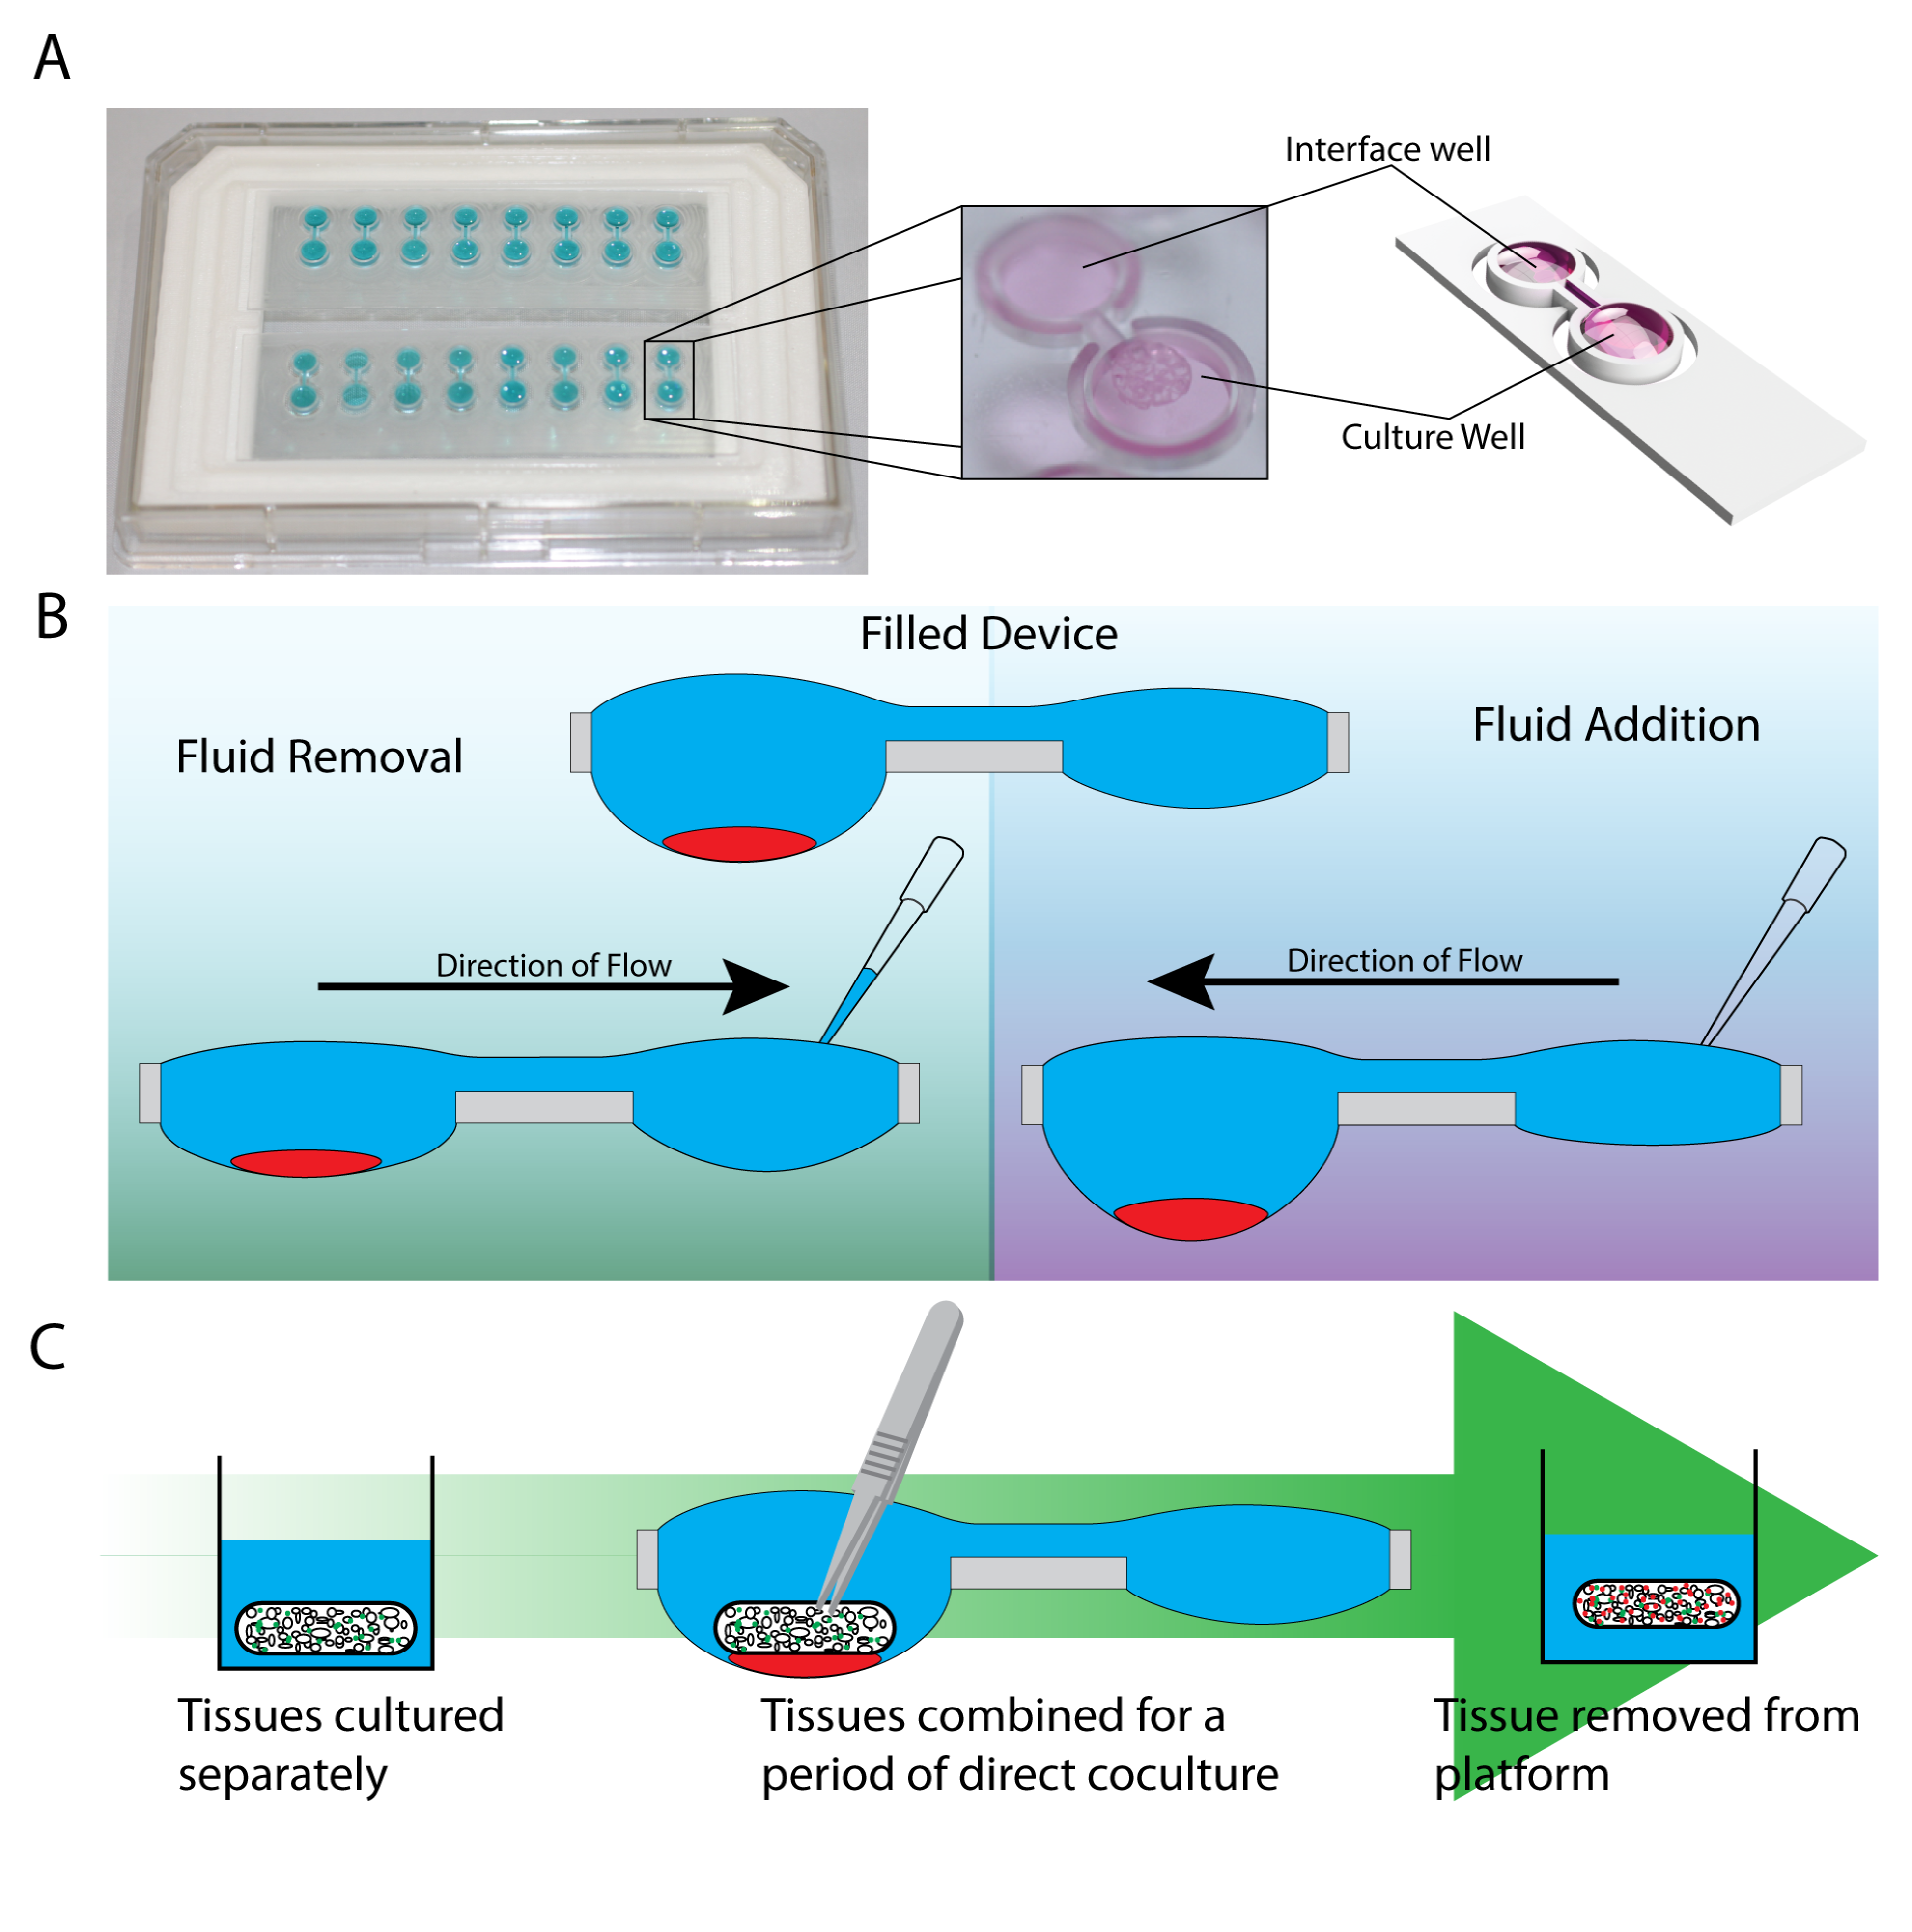
\includegraphics[width=5.4in]{/Figure1-RSC.png}
\caption[\textbf{The two-well hanging droplet device, operation, and capabilities}]{\textbf{The two-well hanging droplet device, operation, and capabilities}. (A) Two 8- device arrays of the two-well hanging droplet device with a close-up image and rendered-model of a single device. (B) Operation of a filled device containing cells, when fluid is removed or added through the interface well, volume of the culture well is changed with minimal disturbance to the culture. (C) Schematic of a dynamic coculutre experiment performed by combining two tissues in the hanging droplet device then separating the tissues.}
\label{figure:Fig1}
\end{figure}


\subsection{Characterization and modeling of two-droplet system}
We developed a numerical model for the behavior of the connected two droplet system to understand the limitations of the system, improve the functionality of the system, and guide the design of suspended droplet systems. The model predicts the distribution of fluid between two droplets as fluid is added or removed from the system. These predicted values were compared to values experimentally acquired in the device (Fig. \ref{figure:Fig2}Ai). Having a range of well characterized values allows the operation of the device with volumes that are robust and do not risk potential modes of failure. At low volumes, the hanging drop follows a surface-tension dominant regime dictated by the Laplace pressure \cite{Walker2002, Berthier2007} in which the two drops are close in volume. At higher volumes, however, gravity is non negligible, and the shape of the drop becomes elongated \cite{Carvajal2011}. Fluid distribution between wells at increasing volumes is illustrated in Figure \ref{figure:Fig2}Aii where the modeled fluid borders of each well at each volume is overlaid on images of the device. 

To predict the behavior of the system during device operation, we created a dynamic model of the device (Fig. \ref{figure:Fig2}B). With the model, we are able to observe that when one of the droplets, typically the droplet in the largest suspended port, becomes the lowest pressure region it acquires the majority of the liquid in the system. The model further shows that adding and removing fluid to the small drop results in approximately the same volume being shuttled to the well containing the largest drop. Importantly, this model validates the use of the small drop as a buffer for fluid additions; the small drop temporarily stores the fluid that was added by pipetting, prior to delivering it to the larger drop. Utilizing this approach, it becomes simple to tailor the delivery rate to the large drop in order to prevent excessive flow by designing the geometry of the channel connecting the two drops appropriately \cite{Berthier2011}. Finally, the model incorporates the dripping volume for a hanging drop, allowing the prediction of the maximum volume that can be added before detachment of the large drop. Alternatively, this can be utilized as a method for collecting the cellular sample; precise volumes of fluid can be added to cause the dripping of the cells in the drop into a receptacle placed below.

\begin{figure}[h!] %DONE
\centering
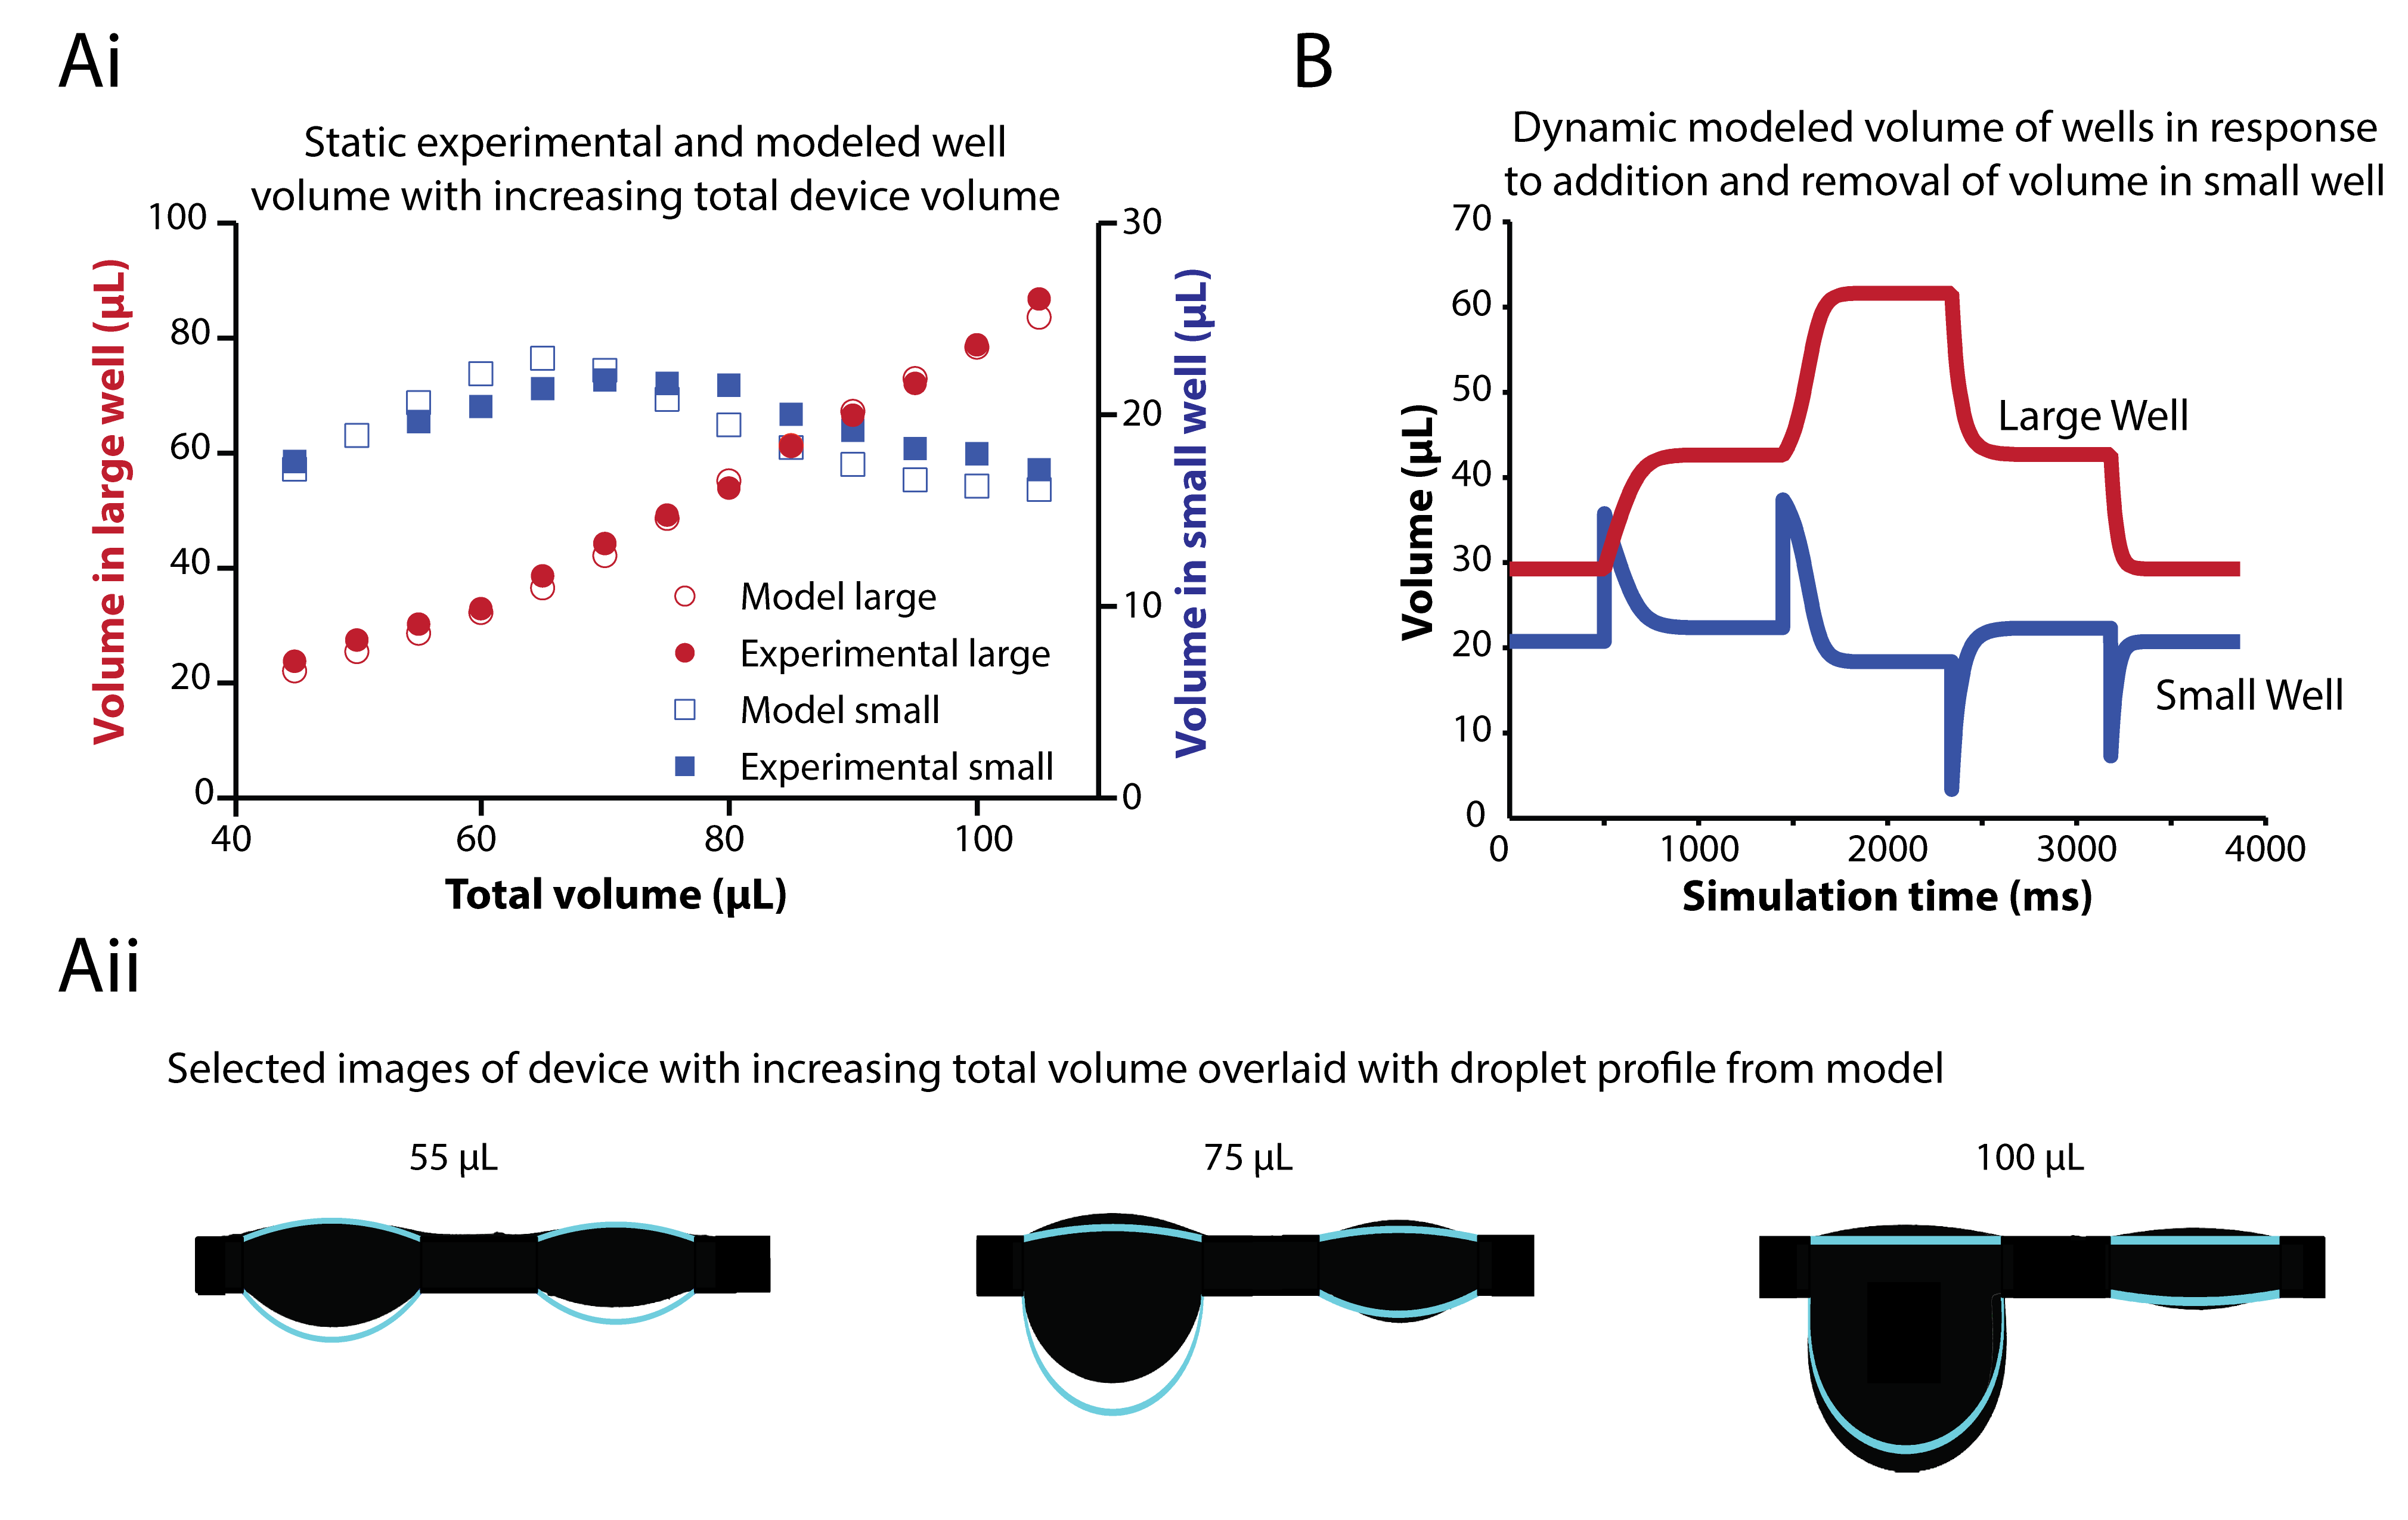
\includegraphics[width=5.75in]{/Figure2-rsc-01.png}
\caption[\textbf{Static and dynamic modeling of volume in each well of the device.}]{\textbf{Static and dynamic modeling of volume in each well of the device.} (Ai) The experimental (solid) and modeled (hollow) volume in each well at steady state with increasing total volume in the device. (Aii) The silhouetted device overlaid with the droplet borders of the modeled system for 55, 75, and 100 μL of total fluid in device. (B) Dynamic modeling of fluid in each well of the device as fluid is added then removed from the small well.}
\label{figure:Fig2}
\end{figure}


\subsection{Two-well hanging drop system prevents shear stress during media exchange}
Shear stress on a cell results in considerable changes to cell behavior \cite{White2007}, including inhibition of apoptosis in some cells \cite{Dimmeler1996} and induced proliferation and differentiation in other types \cite{Yamamoto2003}. In spheroid culture shear can prevent aggregation and completely disrupt the macrostructure of suspension cell cultures. Reducing shear experienced by cells in culture is critical to minimizing undesirable cell stimuli and achieving consistency between experiments. The two-well system provides a reduction in shear stress when changing fluid in hanging droplets compared to a one-well system. We performed an experiment to determine the extent of protection provided by the damping effect for droplet equilibration observed in our model (Fig. \ref{figure:Fig2}). This is best illustrated by a direct comparison between the two- and one-well systems (Fig. \ref{figure:Fig3}). We chose a multiple myeloma suspension cell line, MM.1S (commonly used for multiple myeloma drug studies \cite{Greenstein2003, Tai2006, Azab2009}) for the comparison, because suspension cell lines are generally difficult to culture in microdevices and are easily removed by flow. When cultured in the hanging droplet platform, MM.1S cells settle into clusters but do not form sphereoids. Addition or removal of fluid will result in loss of myeloma cells since the cluster is easily disturbed by minimal force exerted during fluid manipulation. In the hanging drop system media replacement is performed using iterative pipetting steps. Thus, we compared the performance of the two- and one-well systems over multiple pipetting steps.

We designed the experiment to ensure accurate comparison between the two- and one-well systems. The diameter and volume of the culture well in the two-well and one-well system was identical; the volume of fluid removed was based on a fraction (one third) of the total volume in each system. Pipetting was performed by a liquid handling robot to keep the flow rate constant. Each image in Figure \ref{figure:Fig3}A represents a different well subject to different conditions of fluid exchange, and all well images were collected within 10 minutes of pipetting. The two-well system protects cell clusters during fluid exchange after several pipetting steps, while pipetting into the one-well system results in immediate disruption of cluster morphology. These results combined with the data generated from computational modeling of the system underscore the need for an unequal two-well system for suspension cell culture to culture and retain cells to a single well, and suggest that media exchanges in one-well systems may have unintended effects on suspension cell culture.

To evaluate the difference in shear between pipetting into a single-well versus a two-well system, we performed particle image velocimetry (PIV) analysis on fluorescent microbeads in the culture well (Fig. \ref{figure:Fig3}B). Fluid was added \textit{via} the user interface well (in the two-well system) or directly into the culture well containing the fluorescent beads (in the one-well system). There was a 10-fold reduction in the velocity of beads in the two-well device compared to the single-well one. This reduction velocity corresponds to a comparable decrease in shear stress experienced by cells in the device. Furthermore, the reduction in velocity in the two-well system enables quicker media changes without cell disruption, compensates for variation of users operating the device manually, and results in shorter times where the device needs to be exposed (to interface with pipettes), reducing potential evaporation.

\begin{figure}[h!] %DONE
\centering
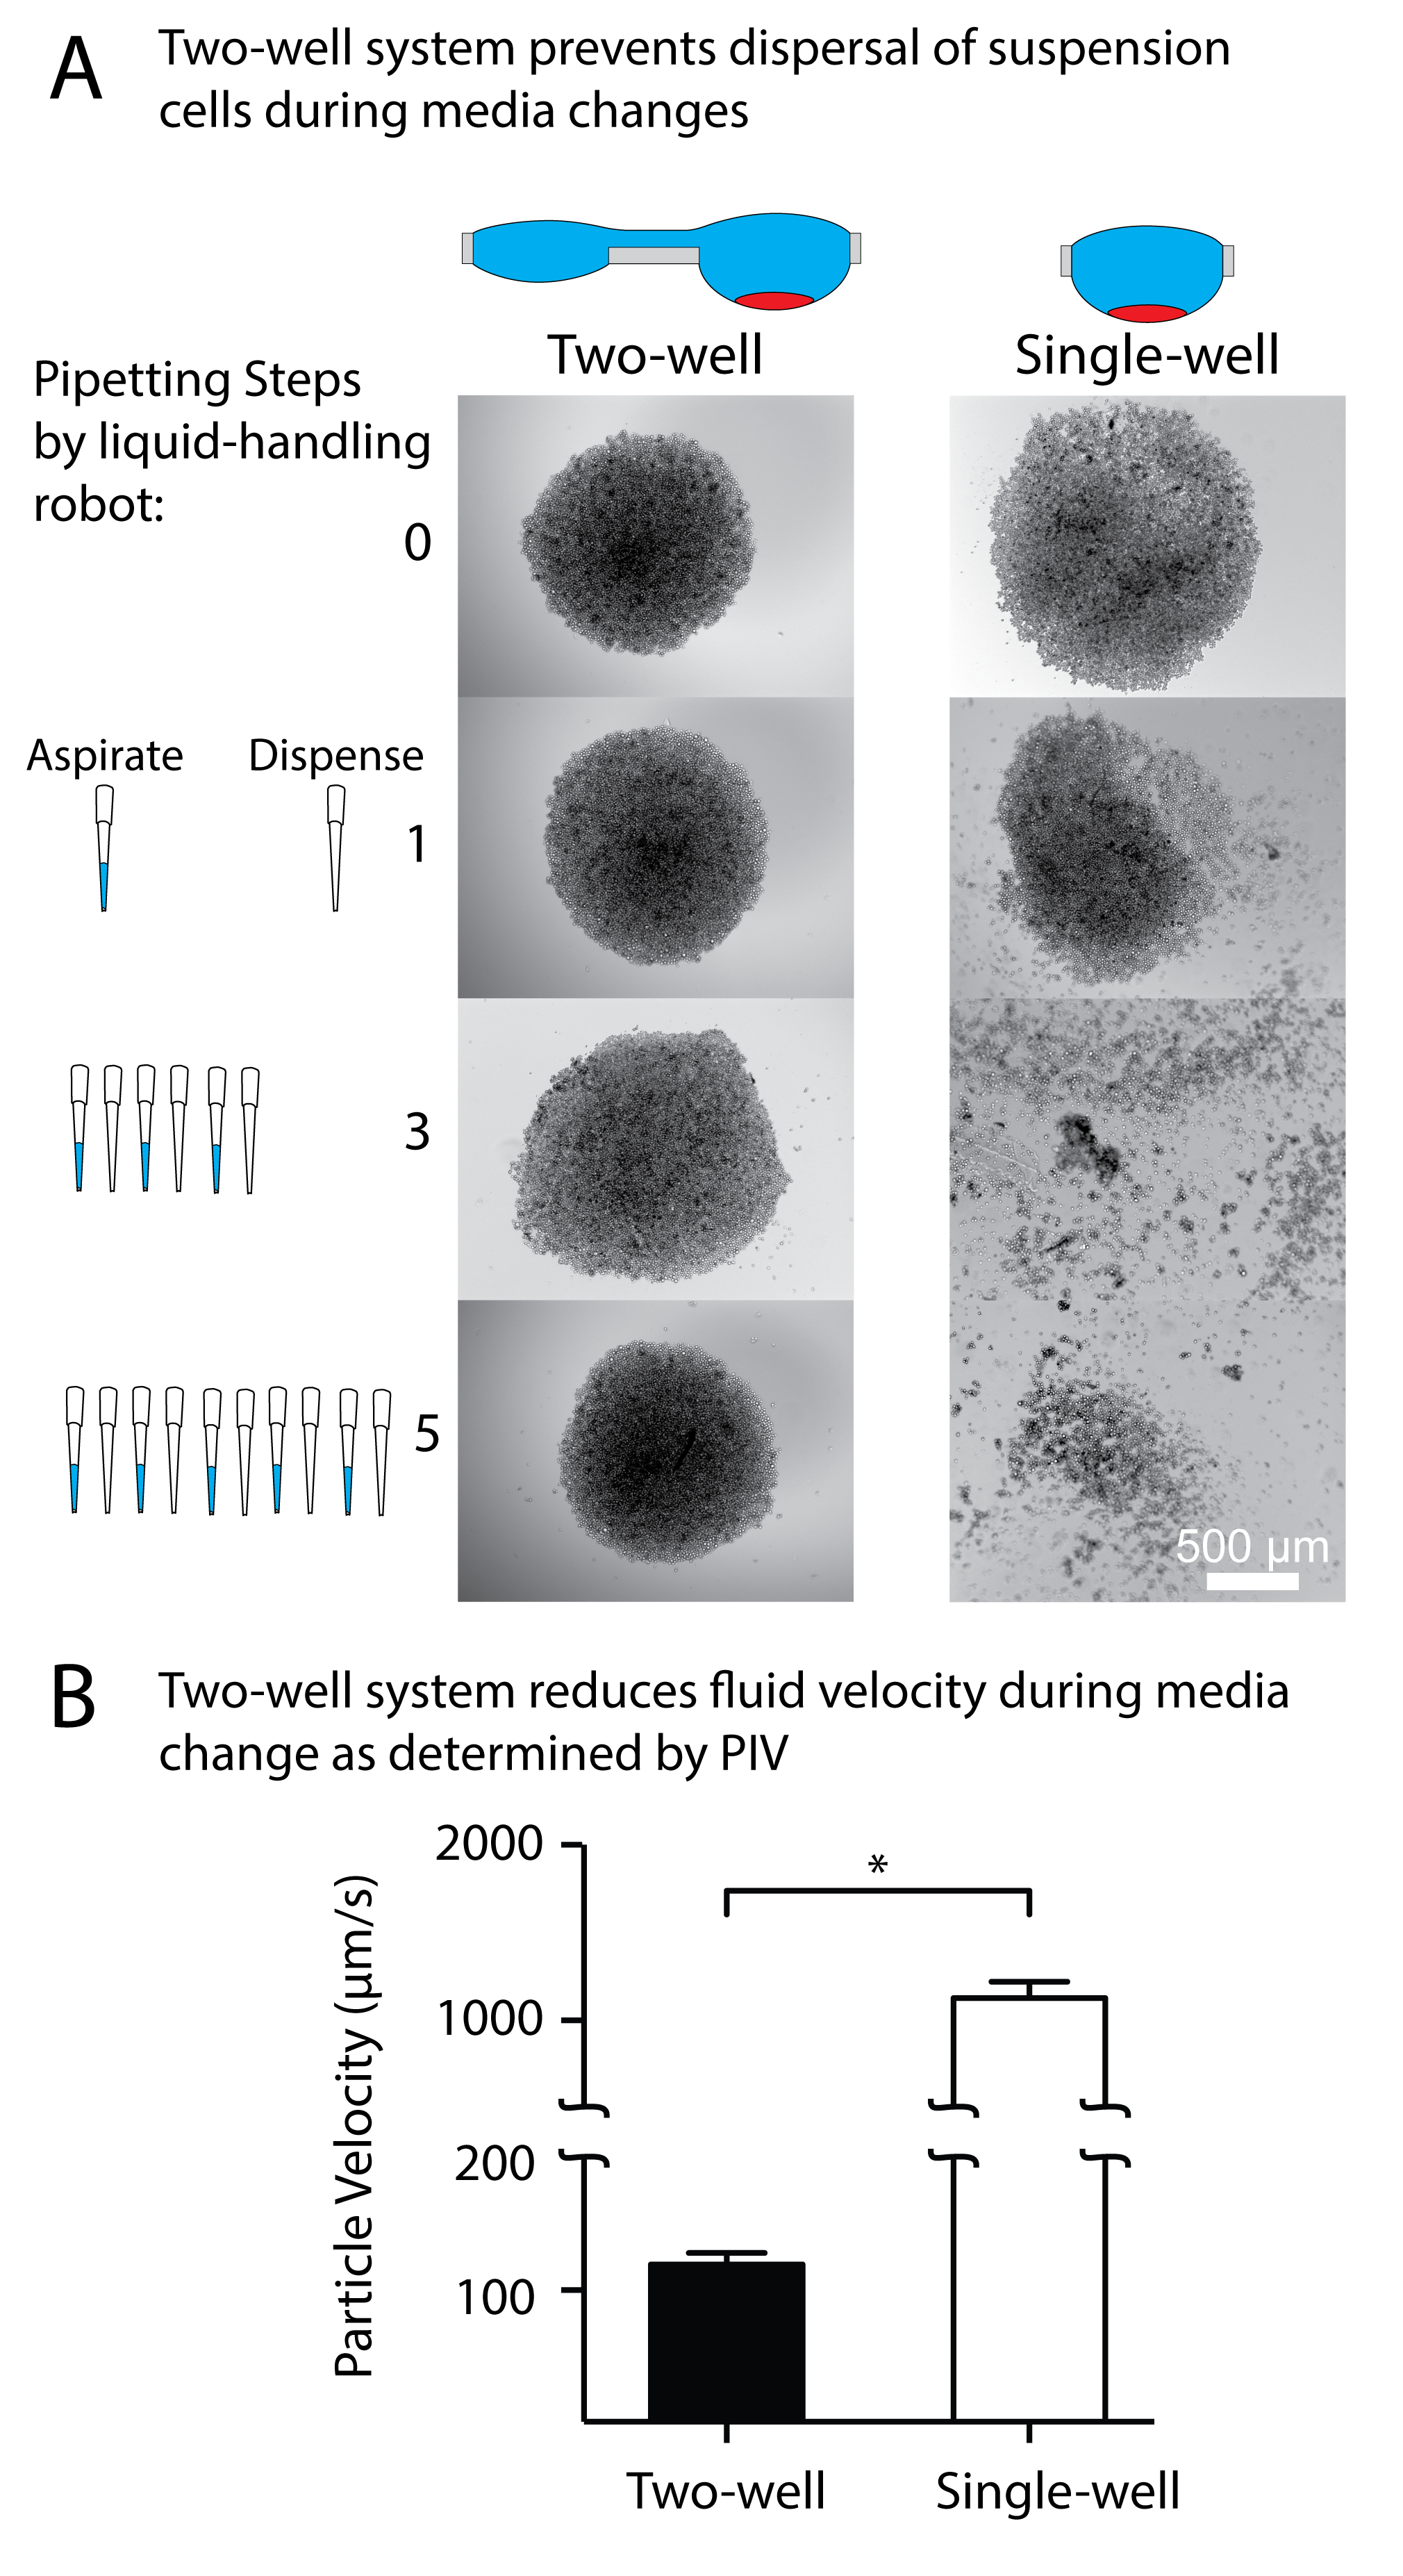
\includegraphics[width=3in]{/Figure3-RSC.png}
\caption[\textbf{Effects of pipetting into a single-well and two-well device}]{\textbf{Effects of pipetting into a single-well and two-well device.} (A) Brightfield images of an MM.1S suspension culture in the device before and following 1, 3, and 5 pipetting steps at 1 mL/min of approximately 33\% of the total media in single-well and two-well device. (B) PIV was used to determine the velocity of fluid at a fixed z position in the culture droplet during fluid addition to the interface droplet (two-well) or directly (single-well). Error bars represent the standard deviation of four replicates (*p<0.0001).}
\label{figure:Fig3}
\end{figure}

\subsection{Open hanging droplet platform facilitates key cell culture manipulations and readouts}
For functional validation, we demonstrated that the hanging droplet culture platform is well suited to perform functions critical for tissue culture, experimentation, and analysis: long-term culture, ability to apply treatment, and immunocytostaining. We chose to focus our cellular validation experiments using suspension (or non-adherent) multiple myeloma cells. Multiple myeloma is the second most common hematopoietic malignancy in the United States, and has a 47\% median 5-year survival rate. Multiple myeloma affects its microenvironment through a complex network of interactions with surrounding matrix and cells resulting in the destruction of healthy bone \cite{Reagan2014} and acquisition of drug resistance \cite{Bianchi2006}. The fact that multiple myeloma cells are non-adherent precludes the use of many currently available microculture platforms for studying the disease.  We performed the platform validation using the multiple myeloma cell line, MM.1S. The MM.1S cell line is an important model for multiple myeloma, and the assays we have focused on are key to studying the disease and patient-specific drug responses \cite{Young2012}.
\newline
\textit{i. Long term culture.} The extended culture experiments were performed over the course of 9 days, feeding the culture every other day through media replacements, resulting in approximately 75\% new media in the culture well each feeding. The MM.1S cells expressed mCherry, which was used to perform a relative quantification of total cells in the well. Mean integrated density of fluorescence signal across the entire well was used because a single cell count was not feasible due to the high density of cells and cell-to-cell variation in mCherry expression levels. Over the course of the experiment (Fig. \ref{figure:Fig4} A), the number of cells increased through day 5, but had stopped by the 6th day. At that time in the culture, the wells had become overpopulated resulting in stagnation of the mean integrated density. Though nine-day culture is rarely required for common experiments such as drug screens, we have demonstrated the practicality of long-term culture in the device. \newline
\textit{ii. Cell viability in response to \textit{in situ} treatment.}

We characterized growth inhibition of the culture in response to a drug to demonstrate the ability to apply treatments during culture and measure a dose-response. We treated MM.1S cells with bortezomib, a proteasome inhibitor and commonly used treatment for multiple myeloma (Fig. \ref{figure:Fig4}B). The IC50 value of the MM.1S culture in response to bortezomib was determined to be 26.2 nM with an R\textsuperscript{2} of 0.84. The previously reported IC50s of bortezomib for the MM.1S cell line typically range between 4 and 9 nM \cite{Bianchi2006, Hu2014, Horton2006}, but these values were all calculated in 2D culture. It has been widely shown that 3D culture conditions often decrease drug sensitivity \cite{Tung2011, Friedrich2009}and better recapitulate in vivo response. The calculated response also for a 24 hour exposure time, follows a distinct 4 parameter logistic sigmoidal curve characteristic of inhibitory dose-response curves. 

\textit{iii. High content assays and immunocytochemistry (ICC)} To establish the viability of functional readouts in the platform, we characterized NF-\textkappa B translocation to the nucleus in MM.1S cells in response to stimulation \textit{via} TNF-\textalpha. Quantifying translocation of factors between cell membrane, cytoplasm, and nucleus of the cell provides a high-content assay that can give information about the state of a single cell or population of cells. Translocation of factors around the cell is a vital component in cell behavior and proliferation \cite{Chuderland2008}. Misregulation of translocated factors, such as estrogen receptor in breast cancer \cite{Revankar2005} and androgen receptor in prostate cancer \cite{Molina2011}, contributes to treatment resistance. In multiple myeloma, NF-\textkappa B has been implicated as key regulator of inflammation, cancer progression, cell survival, and acquired resistance \cite{hideshima2000thalidomide}, and thus is considered as a potential therapeutic target. 

We performed an experiment to induce translocation of NF-\textkappa B in response to TNF-\textalpha  in the MM.1S cell line (Fig. \ref{figure:Fig4}C). TNF-\textalpha  is expected to cause NF-\textkappa B to translocate to the nucleus following treatment and is the first step in the transcription of a number of pro-inflammatory mediators \cite{Pahl1999}. Translocation is indicated by a steeper slope in the scatter plot comparing the mean signal intensity of NF-\textkappa B in the nucleus versus the cytoplasm (Fig. \ref{figure:Fig4}Ci). When considering the entire population of cells using a histogram, a population-wide increase in translocation is visualized as a shift to the right on the x-axis (mean nuclear NF-\textkappa B signal intensity to mean cytoplasmic NF-\textkappa B signal intensity) with a median shift from 1.0 in the untreated condition to 1.2 in the treated conditions with p<0.001 from analysis with the Mann-Whitney U test for 4 replicates (Fig. \ref{figure:Fig4}Cii).

\begin{figure}[h!] %DONE
\centering
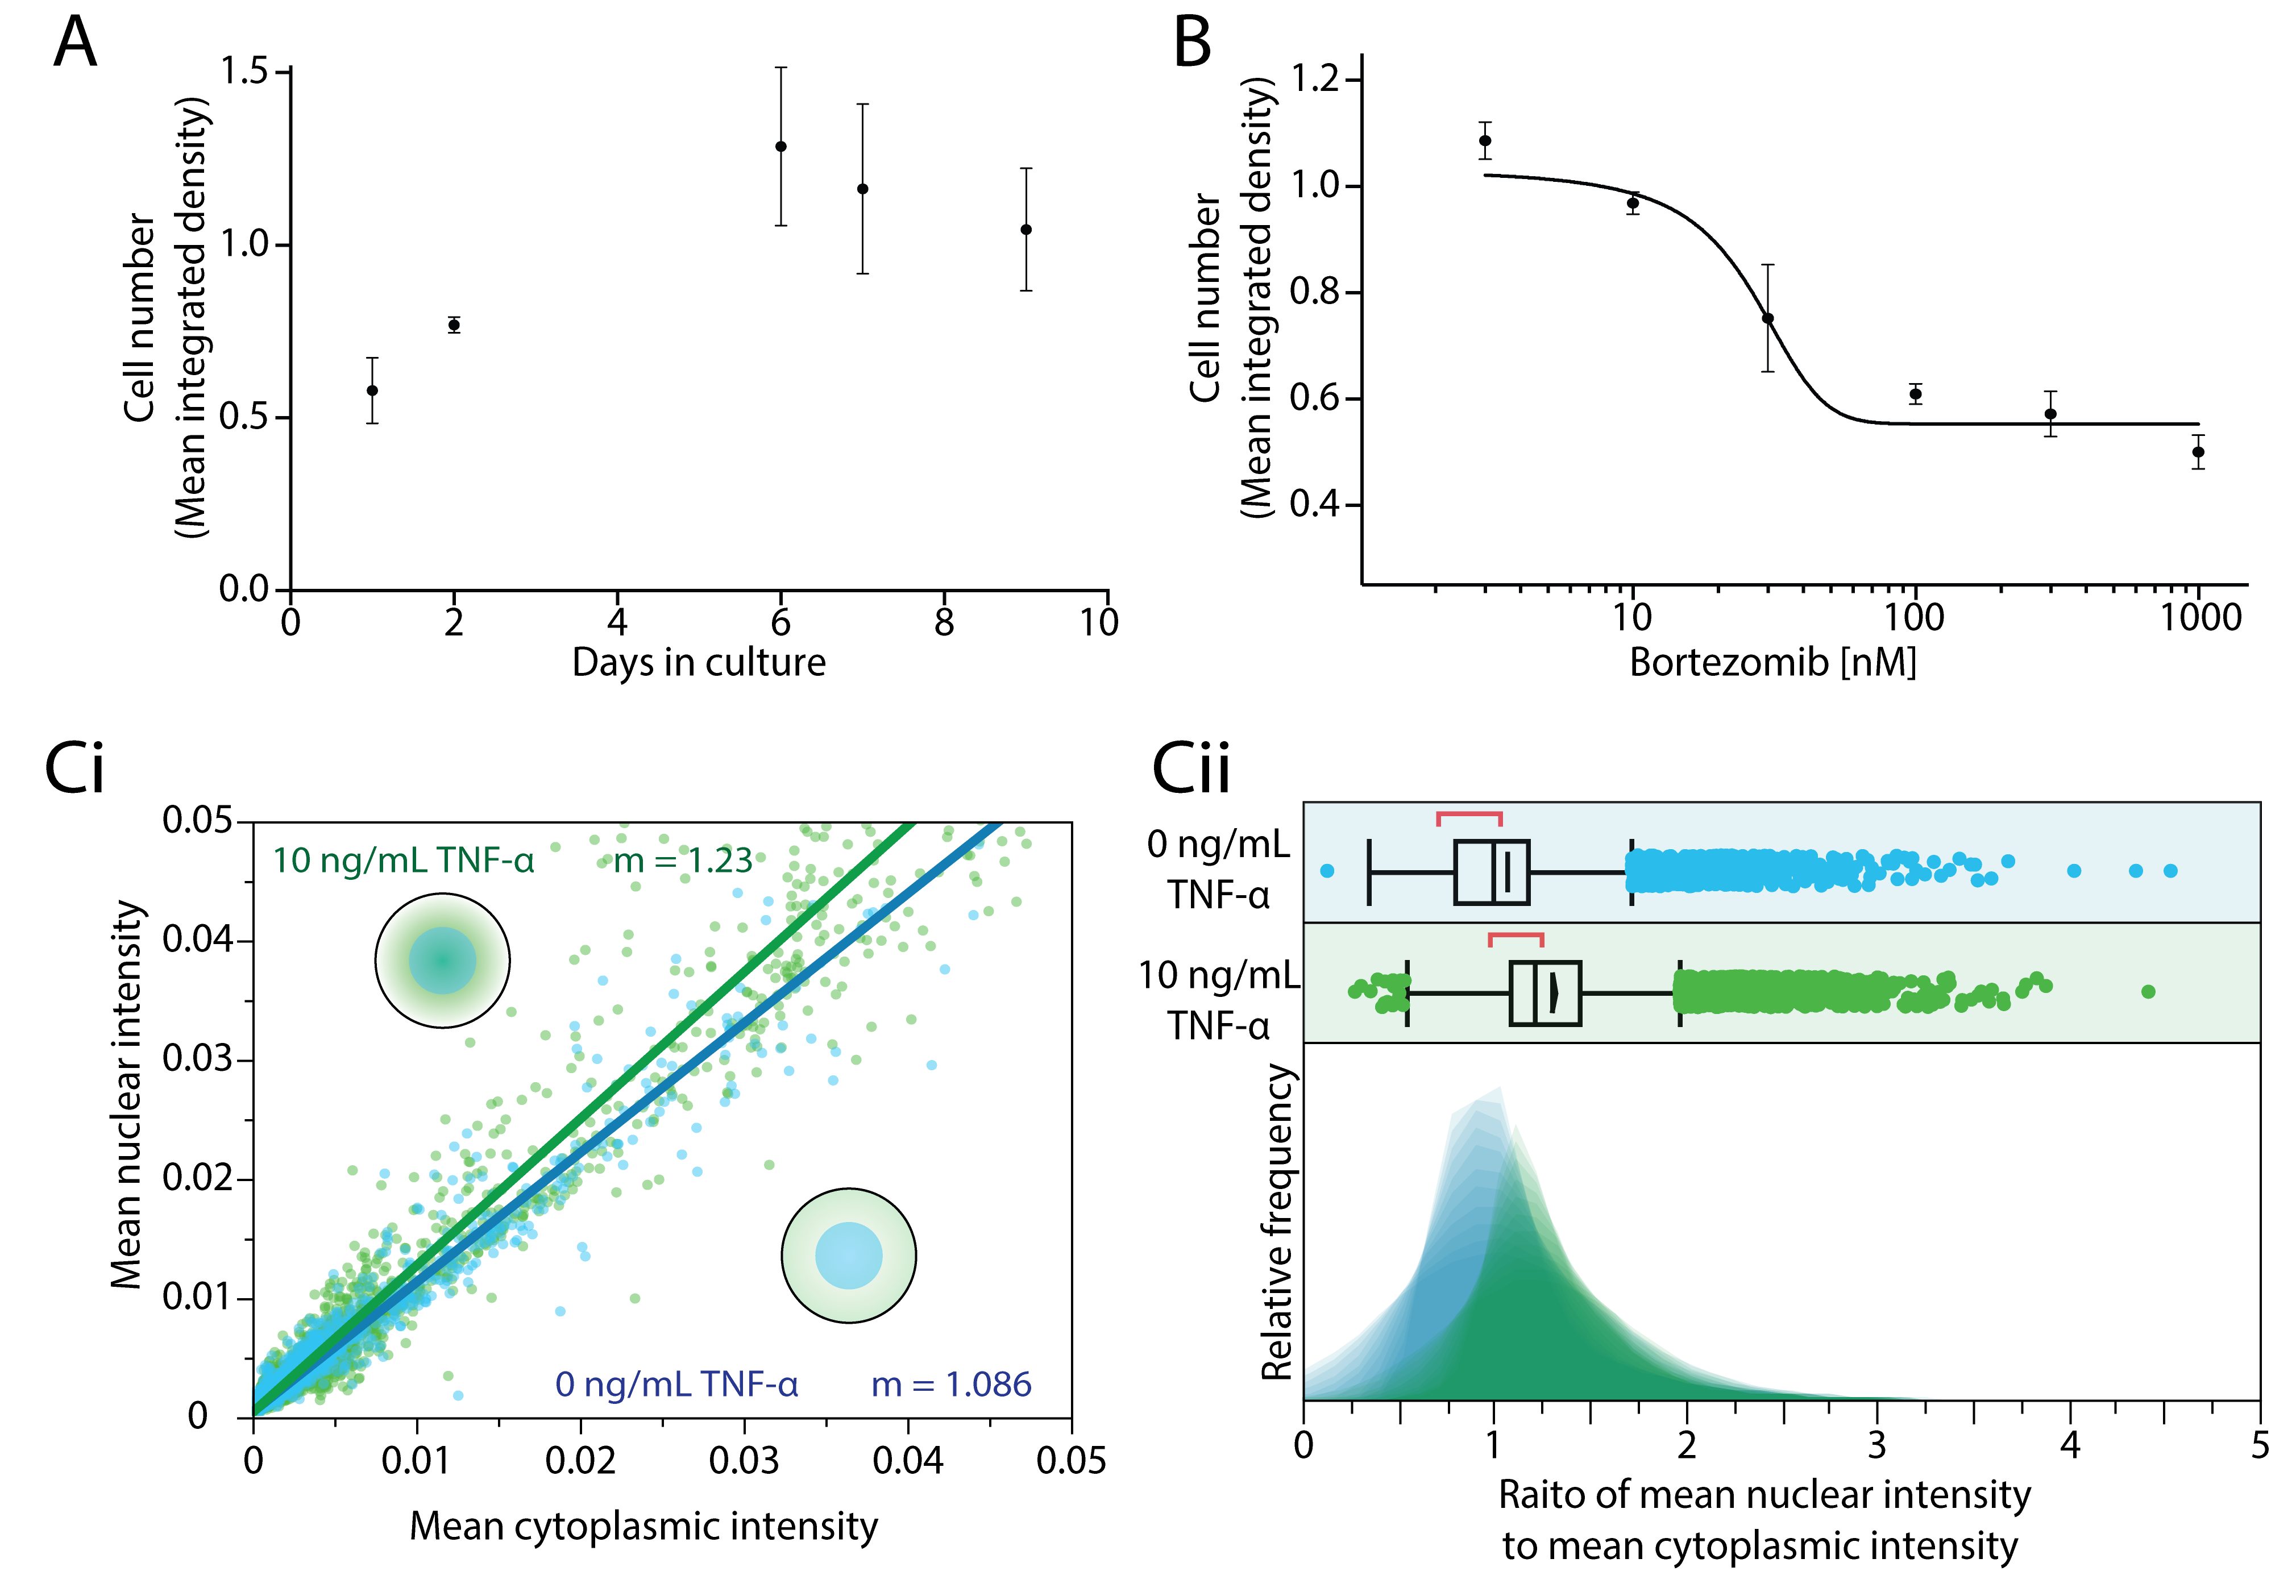
\includegraphics[width=5.75in]{/Figure4-RSC.png}
\caption[\textbf{Open hanging droplet platform facilitates key cell culture manipulations and readouts.}]{\textbf{Open hanging droplet platform facilitates key cell culture manipulations and readouts.} (A) Long term culture: Growth of MM.1S cells in device across a 9-day culture. Error bars represent the standard error of the mean (SEM) of 7 wells. (B) Cell viability assays in response to in situ treatment: Growth inhibition response curve of MM.1S cells to increasing concentrations of bortezomib in culture. Error bars represent the SEM of 5 wells. (C) Characterization NF-\textkappa B nuclear translocation in MM.1S cells following treatment with 10 ng/mL of TNF-\textalpha \, (green) or no treatment (blue). (Ci) Scatter plot of mean nuclear intensity versus mean cytoplasmic intensity. (Cii) Histograms of the ratio of mean nuclear intensity to mean cytoplasmic intensity for the population of cells.}
\label{figure:Fig4}
\end{figure}

For the NF-\textkappa B translocation assay described above, we developed methods to perform ICC on cells from hanging drop cultures. We first attempted to perform ICC in situ (i.e., in the hanging droplet device), leveraging the two-well system to exchange ICC reagents. However, performing ICC requires a permeabilization step using surfactants, which inherently reduce interfacial tension. Standard in situ ICC was found to be incompatible with the hanging droplet device due to the reliance on pressure equilibration to move fluid between wells. When surfactant is added to the user interface well  the surface tension decreases, causing a shuttling of fluid from the culture well into the interface well. To achieve high-content ICC in the NF-\textkappa B translocation assay, we instead transferred the cells from the hanging droplet wells to a poly-L-lysine-treated slide to retain cells during fluid exchange by touching off the droplets onto the surface of the slide.  Performing ICC and imaging on plated cells has several advantages compared to in situ ICC and imaging. The cells are spread throughout the plate, allowing for better separation of cells and therefore better characterization of single cells to be achieved. Plating cells also enables higher objectives to be used for imaging and longer imaging times to be achieved. In the current configuration, devices would need to be removed from the humidifying dish to be accessed by high magnification objectives due to working distance limitations. 

It is worth noting that other staining protocols that do not require surfactants, such as live/dead assays, can be performed directly in the hanging droplet device. We demonstrated this using the adherent cell line MDA-MB231, which forms spheroids in hanging droplet culture (Fig. \ref{figure:FigS2}). We incubated the device in both normoxic and hypoxic conditions to study the spatial distribution of live and dead cells within the spheroid. Live/dead staining was performed within the hanging droplet device, and the spheroids were removed for imaging (Fig. \ref{figure:FigS2}). 
\newline
\textit{iv. Culture treatment, media sampling and cytokine quantification}The ability to sample and analyze media throughout the course of an experiment without disturbing the culture is powerful for studying progression of a culture system. The two-well system is well-suited for media collection and treatment addition through the interface well. To validate the platform for treatment and sampling, we cultured a polymeric porous bone-like scaffold seeded with bone marrow stromal cells in the device. The scaffolds were treated at seeding and after 24 hours with AMD3100, an inhibitor of CXCR4, indicated in homing and adhesion for cells to the bone marrow microenvironment \cite{Alsayed2007, Burger2006}. The media was sampled at 24 and 48 hours from the interface port and analyzed for the pro-inflammatory, IL-6 cytokine indicated in microenvironment-mediated drug resistance and a number of pro-tumorigenic pathways \cite{Hodge2005, Roodman2001a, Vincent2005, Lin2007}. IL-6 was detected in both the control and AMD3100-positive conditions when sampled from the interface well (Fig. \ref{figure:Fig5}A). As expected, we observed a trend toward reduced IL-6 secretion with AMD3100 treatment. This experiment demonstrates that cytokines secreted by cells in the culture well are able to be detected in the interface well and suggests that this device could provide a useful tool for conducting soluble factor signaling-based coculture experiments using more complex culture constructs. We further evaluated soluble factor exchange in the device through computational modeling of diffusion in the system starting with an initial concentration of a molecule with similar diffusion properties to IL-6 in the volume occupied by the bone-like scaffolds (Fig. \ref{figure:Fig5}B). At 4 hours, the diffusion gradient stabilizes within the culture well of the device creating a pattern where the culture well has a stable "high" concentration and the interface well have a stable "low" concentration of the solute. Further characterization of diffusion within the device is available in the ESI (Fig. \ref{figure:FigS3}).    

\begin{figure}[h!] %DONE
\centering
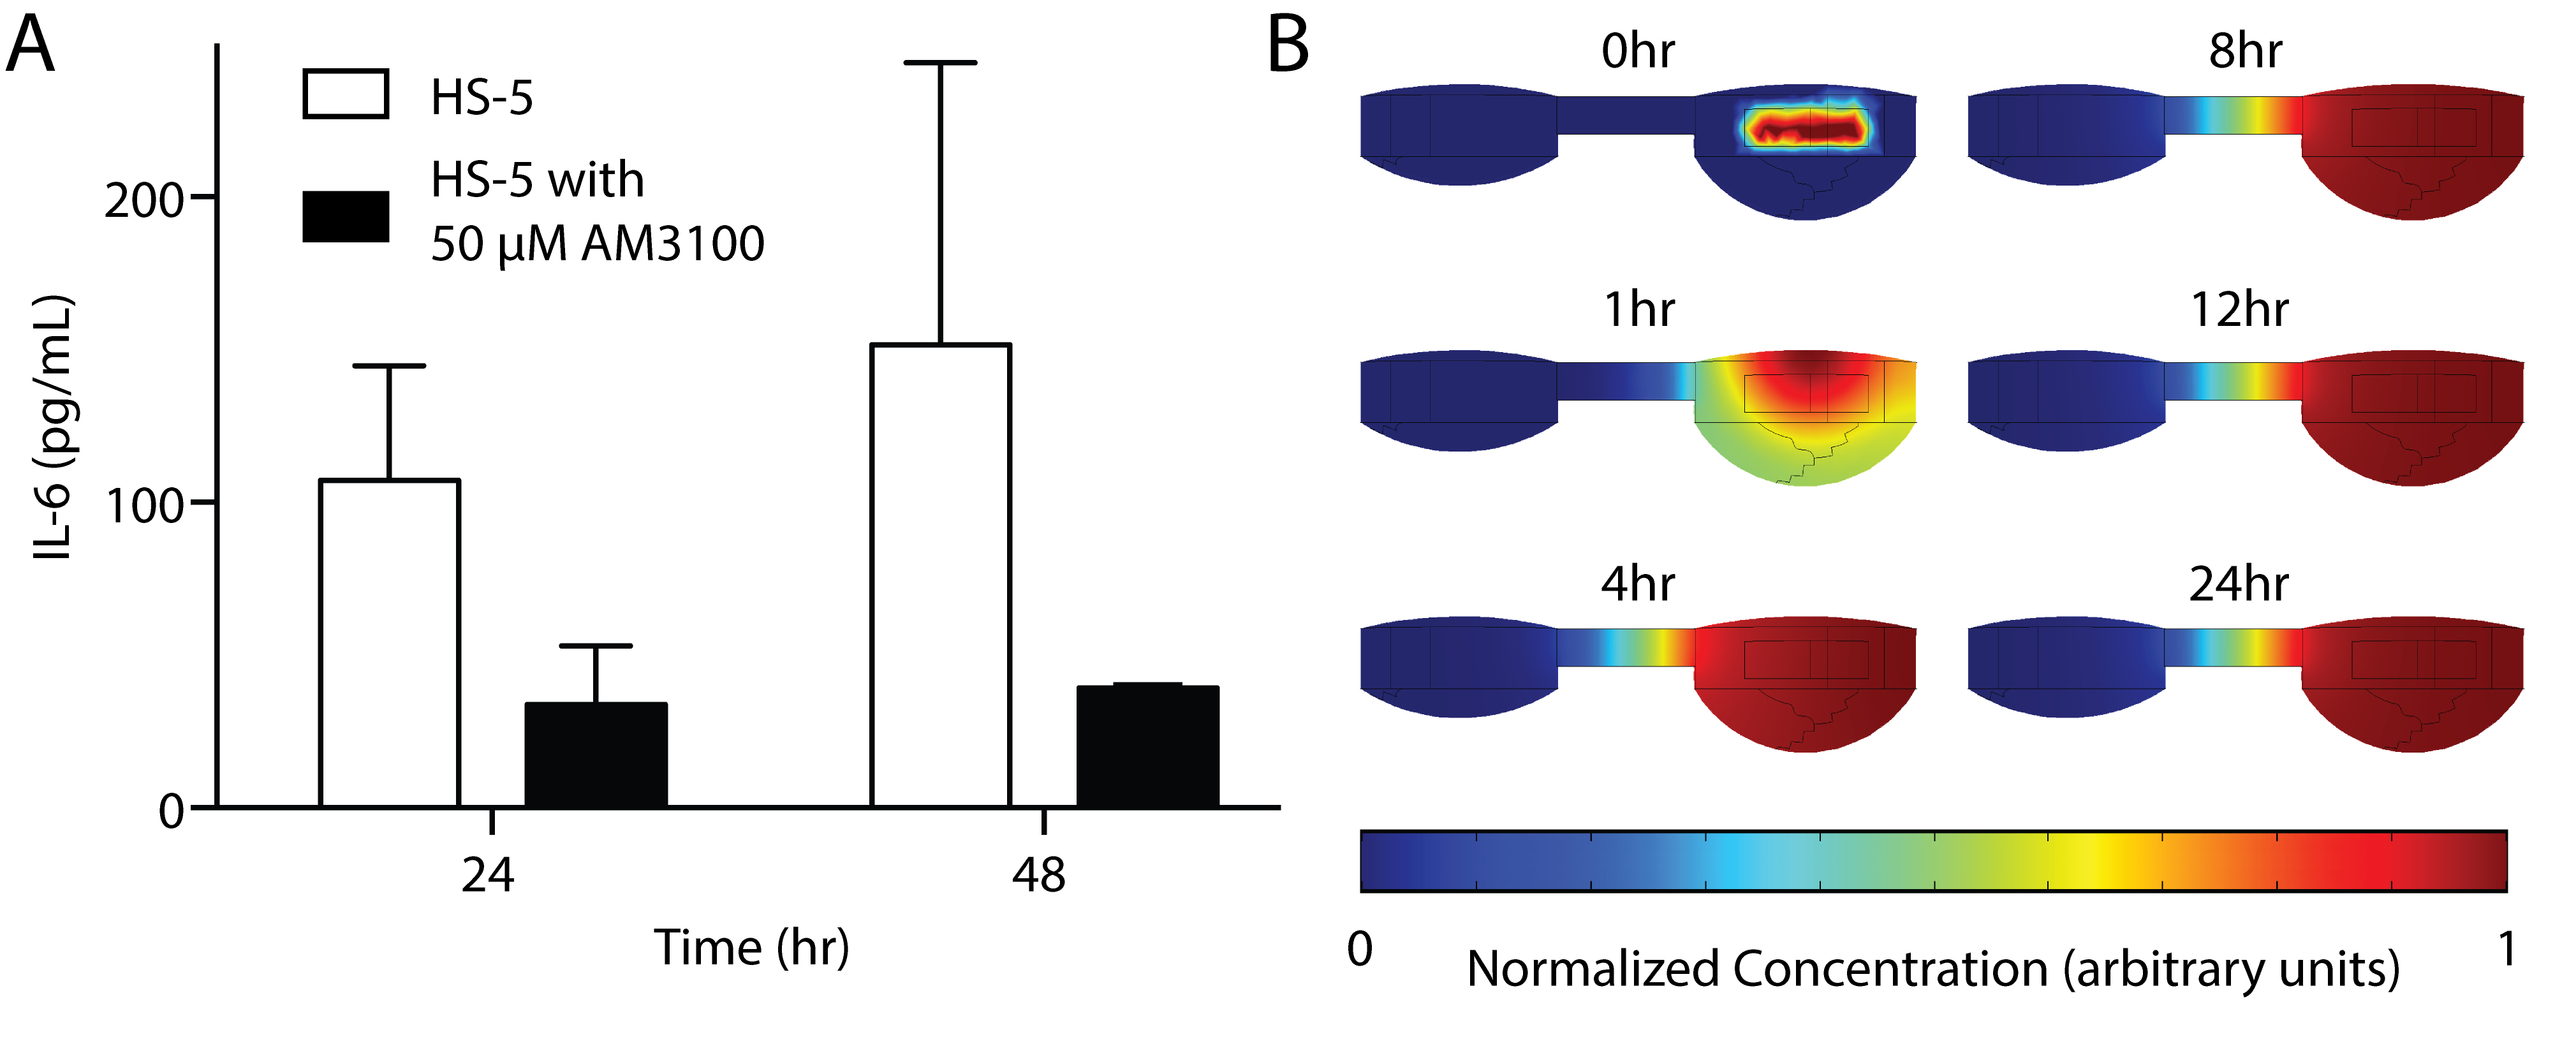
\includegraphics[width=5.75in]{/Figure5-RSC.png}
\caption[\textbf{Soluble factors in culture.}]{\textbf{Soluble factors in culture.} (A) Concentration of IL-6 isolated from HS-5-seeded bone-like scaffolds cultured in device taken from the interface well at 24 and 48 hours of culture. Error bars represent the SEM of 3-4 wells. (B) Plot of normalized concentration for simulated diffusion in the device at several time points over 24 hours. The initial concentration of solute was localized to the volume occupied by the bone-like scaffold at time = 0 h. The solute simulated was approximately 10 kDa with a diffusion coefficient of 100 \textmu m\textsuperscript{2}/s.}
\label{figure:Fig5}
\end{figure}


\subsection{Dynamic culture of cells and tissue scaffolds}
The geometry of the device allows for direct access to the culture through the open wells. This access can be exploited to manipulate culture throughout the course of an experiment. We demonstrated manipulation of the media through the wells (sections 3.3 and 3.4), importantly, the open system facilitates interaction beyond simple media changes and liquid treatments. As shown in Fig. \ref{figure:Fig1}, tissue scaffolds and solid objects can be introduced \textit{via} direct access to the culture well (e.g., by using tweezers to place the scaffold in the open device). To explore the ability to manipulate tissue throughout the course of an experiment, we performed a coculture of multiple myeloma and bone marrow stromal cells (BMSCs). BMSCs play an important role in multiple myeloma progression and provide the tumor with protection against treatment \cite{Chauhan1996, Chatterjee2002a}. Adhesion of multiple myeloma cells to the stroma is an important step in disease progression as non-malignant B-cells have very low capacity for adhesion \cite{Tai2006}.

We began the culture separately, with BMSCs in polymeric, porous, bone-like scaffolds and myeloma seeded into wells in the hanging droplet device. The cultures were combined in the hanging droplet device and myeloma cells were allowed to migrate into the scaffold. The scaffolds were removed for imaging following coculture and adhesion of MM.1S cells was characterized (Fig. \ref{figure:Fig6}). Adhesion of the MM.1S cells to the scaffold was seen in both direct coculture, where the scaffold and MM.1S cluster were in the same well, as well as in the blank scaffold MM.1S monoculture condition. MM.1S cells were not detectable in either BMSC monoculture or separate coculture. These results enable us to explore the impact of the multiple myeloma microenvironment for both soluble factor signaling as well as cell-cell contact for tumor-stromal interactions. 

\begin{figure}[ht] %DONE
\centering
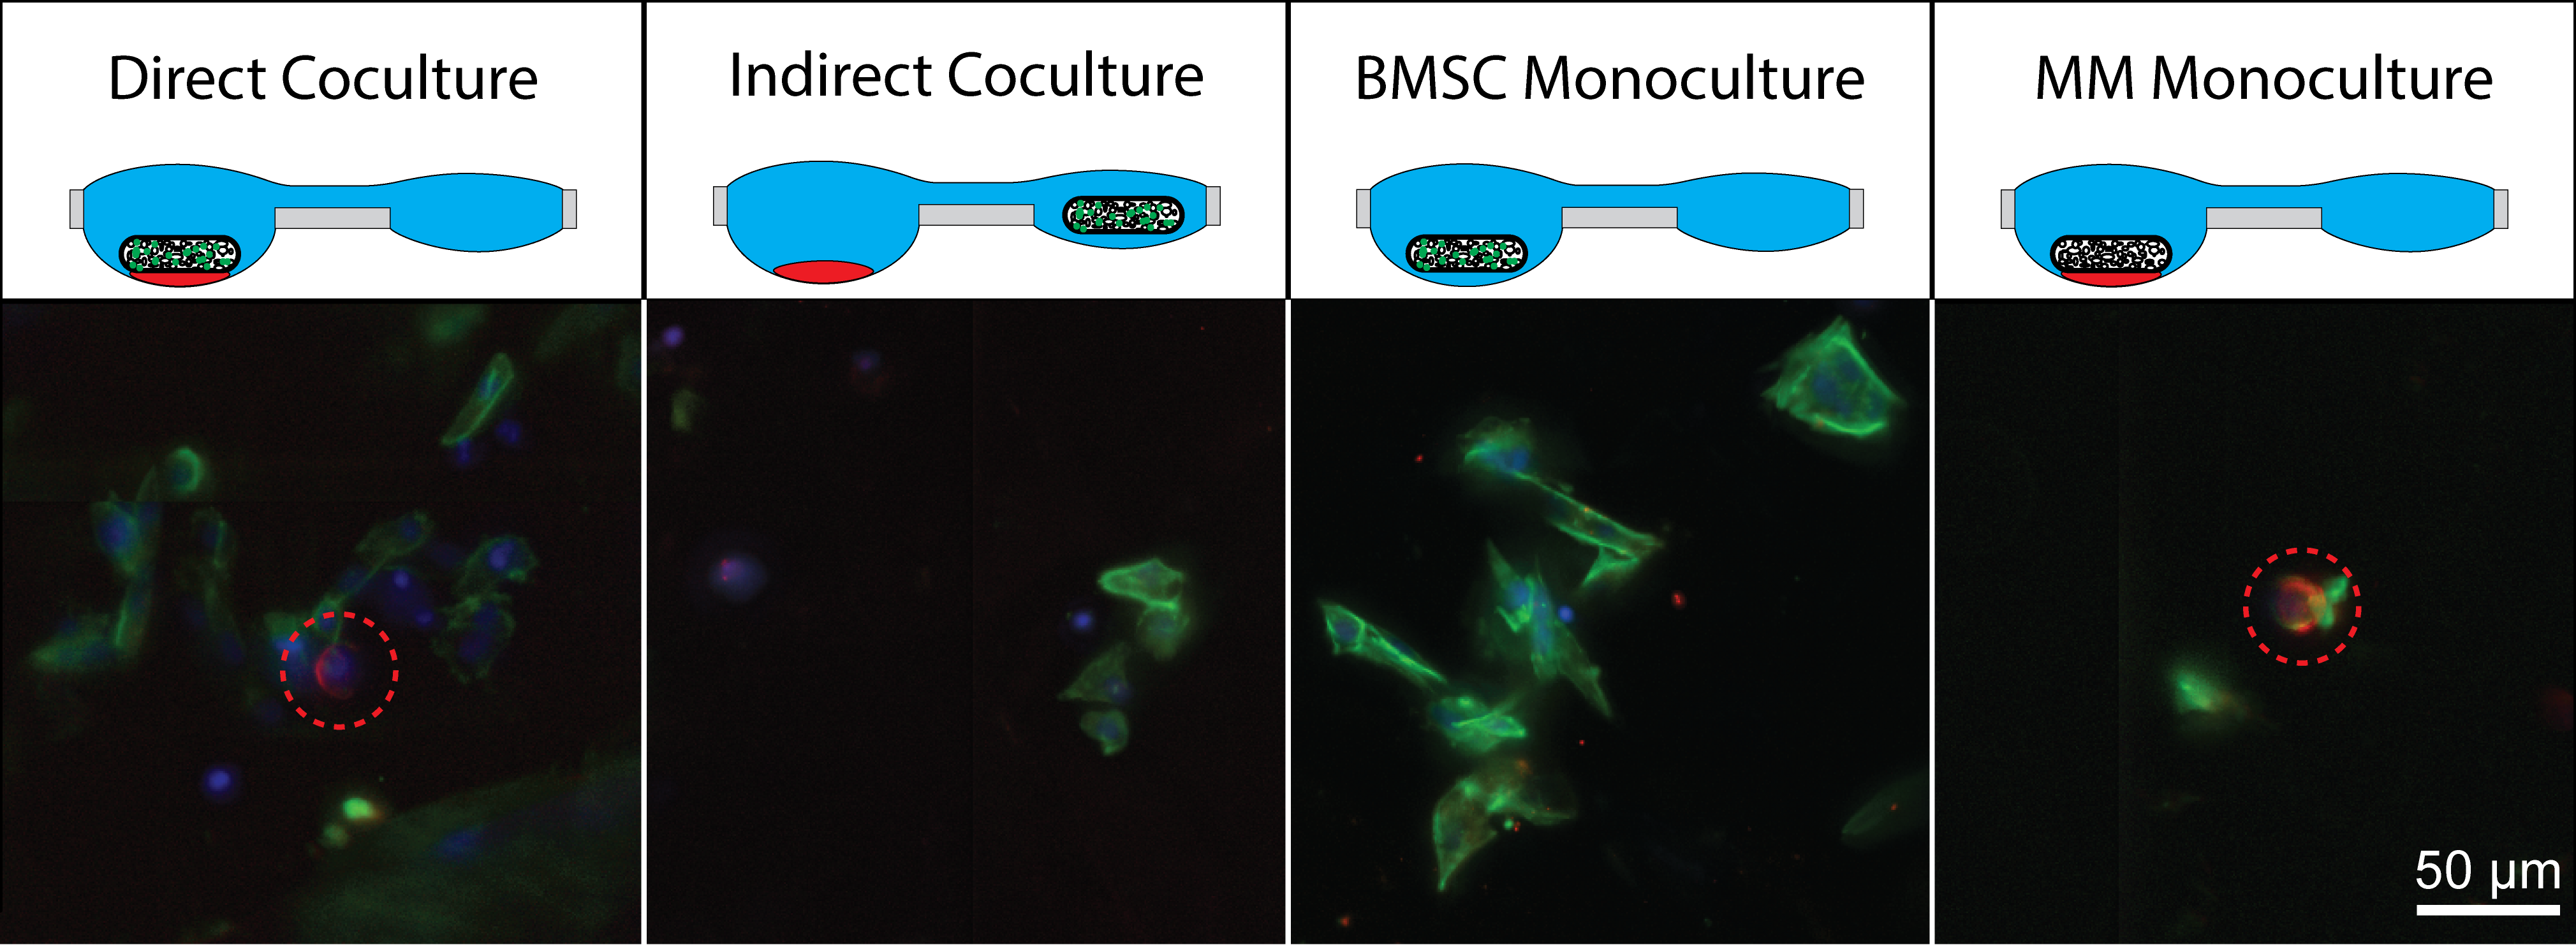
\includegraphics[width=5.5in]{/Figure6-RSC.png}
\caption[\textbf{Coculture and migrations of MM.1S cells into polymeric bone-like scaffold.}]{\textbf{Coculture and migrations of MM.1S cells into polymeric bone-like scaffold.} Fluorescent images of polymeric bone-like scaffolds following either direct coculture (BMSC-seeded scaffold with MM.1S cluster - same well), indirect coculture (BMSC-seeded scaffold with MM.1S - separate wells), BMSC monoculture (BMSC-seeded scaffold only), or multiple myeloma monoculture (MM.1S cultured with blank scaffold). BMSCs were identified by presence nuclear stain (blue) with actin (green), while MM.1S cells were identified by nuclear stain, actin, and CD138 ring (red) and highlighted with a red dotted circle.}
\label{figure:Fig6}
\end{figure}


\section{Conclusions}
We have developed an open platform that enables the dynamic culture and analysis of tissues in a hanging drop embodiment. We have demonstrated that an asymmetric two-well droplet system enables the long-term culture of shear-sensitive cells while allowing for the application of treatments over the course of an experiment. Leveraging the open surface of the hanging drop wells, we are able to add and remove tissue from the culture platform during the course of an experiment to enable dynamic coculture configurations, which are difficult to achieve in closed culture platforms and facilitates easy downstream analysis of cultures. The platform addresses challenges of culturing suspension cells in 3D culture as well as coculture with adherent cell types. The platform enables configurations of cells that were previously either unachievable or impractical, allowing for the investigation of new biological phenomena. We will continue to explore the biology enabled by this platform with the development of more complex biological tissues formed with step-wise, dynamic component addition. 

\section{Acknowledgements}
The authors would like to thank Drs. Shigeki Miyamoto and Fotis Asimakopoulos for their expertise and biological insight into multiple myeloma, Dr. William Murphy and Eric Nguyen for their contributions to in situ imaging in the  and bone marrow scaffold development, and Dr. Jay Warrick for his assistance in PIV analysis. This work was funded by University of Wisconsin Carbone Cancer Center Support Grant P30 CA014520 and National Institutes of health grants; NIH R01 CA155192 (D.J.B.), NIH T32HG002760 (T.E.d.G.), NIH K12 DK100022 (A.B.T.). T.d.G. has ownership in Stacks to the Future, LLC and Lynx Biosciences, LLC. E.B. has ownership in Stacks to the Future, LLC and Tasso, Inc.   D.J.B. has ownership in BellBrook Labs, LLC; Salus Discovery, LLC; Stacks to the Future, LLC; and Tasso, Inc. A.B.T. has ownership in Stacks to the Future, LLC.

\chapter{Stacks for the multiple myeloma microenvironment}
\label{Chap:Stacks}

\section{Introduction}
Let's talk about how great stacks is ok.
\section{Methods}
Filler

\subsection{Fabrication}
We used a mill, then we used injection molding, polystyrene was used and then polypropylene.

\subsection{Device operation}
Filler

\subsection{Multiple myelolma culture}
Filler

\section{Results and discussion}
Filler 

\subsection{Stacks physics}

Discuss spontaneous capillary flow here. At first we used polystyrene then we switched to polypropylene since the conditions for spontaneous capillary flow are dependent on surface contact angle, and the surface contact angle of water any polystyrene is much lower than that of water and polypropylene.

The distribution of fluid in stacks should behave similarly to double-sided open well \cite{DeGroot2016}. At lower volumes, fluid is evenly distributed between the top and bottom of the well. As more fluid is added and the mass of the system increases, fluid is pulled downwards in the direction of gravity and becomes elongated \cite{Carvajal2011}, the end result is a well with a small sessile drop on the top side, and larger pendant drop on the bottom that makes fluid replacement from the top difficult with only one stacks layer. A solution to this issue is to use an additional stacks layer placed on top as a means to change media. The layer fluid exchange layer would be filled with media and then placed on top of the stacks culture where fluid exchange happens through diffusion. Additional fluid exchange steps require the removal of the exchange layer from the assembled device, replacing the fluid in the exchange layer and reassembling the device. We found that slightly altering the geometry of the device eliminates the need for an exchange layer in many cases. If the diameter of the well is slightly bigger at the top of the well than at the bottom it will lower the relative pressure of the droplet on top compared to that on the bottom at low volumes. As volume is increased in this system the one of the principal radii of the larger droplet will continue increasing relative to the bottom droplet further decreasing pressure in the top droplet resulting in fluid added to the system collecting on top of the stacks device or assembly instead of at the bottom. Simply having a slightly larger radius on the top of the device than on the bottom facilitates fluid exchange on top of the device without the necessity for an additional fluid exchange layer.


%% Start the appendices:
\appendix       % Chapters, sections are now appendix style
\counterwithin{figure}{chapter}
\chapter{Open Microfluidics for Education}
\label{App:OpenMicrofluidics}

\section{Introduction}

\subsection{Big trouble in little channels}
Microfluidics can be a scary word for many people. Mention microfluidics to someone who has never heard the term before and there will be nothing but blank faces. Discuss it with those slightly familiar with the field and responses can include responses like, "magic", "that sounds hard", and "uh huh". The word, microfluidics to those doing microfluidics research will conjure images of rows of pumps, tangled webs of tubing, and the dreaded experiment-destroying bubbles.

In 2009, Holger Becker lamented that microfluidics was just to immature of a technology to have a "killer app" and break into the mainstream and predicted that it would be at that point sometime between 2014 and 2019 \cite{Becker2009HypeMicrofluidics}. In 2014, Theranos Inc. achieved a \$9 billion valuation with the promise that it would revolutionize the blood testing industry, being able to perform dozens of assays from a single finger prick, and it was all achieved through microfluidics. It appeared as Becker's prediction was correct and microfluidics was finally beginning to enter the popular lexicon. The public's positive association with microfluidics was short lived as Theranos was unable to deliver accurate results on any of the assays it was developing. The company lost its massive valuation, has been sued, sanctioned by the FDA, and is now subject of a film starring Jennifer Lawrence as the company's founder, Elizabeth Holmes \cite{Stockton2016}. The lack of public understanding of what microfluidics is combined with the negative media coverage can lead one to the conclusion that the field of microfluidics has considerable public relations issues. While being unpopular is not inherently bad for microfluidics, a negative public opinion on the field is. Negative public opinion could lead potential researchers away from microfluidics research and possibly endanger the future of funding in the field. In the current climate the next "killer app" enabled by microfluidics will need to have its inner-workings deeply hidden from view and would do well to avoid using "microfluidics". Microfluidics needs to change its perception to continue to grow and advance.

\subsection{Teaching with microfluidics}
An approach to get people to understand microfluidics principles and get them excited about the subject is the use of classroom educational tools. These tools can be as mundane as the a classroom lecture, involve student-level device fabrication like gelatin (Jell-O) microchannels \cite{Yang2013}, or can give students the full microfluidic blackbox experience with complete pump-driven systems capable of doing droplet microfluidics from companies like Dolomite. Modular systems like breadboard microfluidics have also been introduced to educational settings, however, they also have high entry costs and require extensive setup and preparation time \cite{Chen2011, Shaikh2005, Chen2014, Langelier2011, Papautsky2008}. Each technique has advantages, unfortunately the techniques that result in the highest level of student engagement involve the most effort from the instructor to prepare or are prohibitively expensive for many programs \cite{Fintschenko2011Education:Laboratory}. 

We present a modular microfluidic platform that aims to teach students many microfluidics principles in a hands-on learning environment that maximizes student engagement while reducing instructor effort and institutional cost. The platform utilizes the high surface tension of water at the air-liquid interface and capillary action to drive fluid flow through across open microchannels. The microchannels are engineered onto the surface of modular interconnectable blocks to create microfluidic circuits as described in Chapter \ref{Chap:OpenMicrofluidics}.

\section{Methods}

\subsection{Device design and fabrication}
The microfluidic channel design and block interface are discussed in Chapter \ref{Chap:OpenMicrofluidics}. The blocks themselves are designed to interface and exchange fluids without bonding or any permanent connections so they can reconfigured during operation, reorganized by the user to achieve different functions, and reused for future learning experiences. The choice of a Lego-based interface for the  blocks was designed to be simple to use, and familiar so little training on the part of the instructor and student were needed to learn how to interact with the blocks and create microfluidic circuits. Each of the blocks were designed to perform a microfluidic function. The functions included in the study are dispensing, mixing, valving, combining, and splitting. These basic functions can be used to create an array of different microfluidic circuits capable of achieving different goals. 
Also included in this study was the cross section channel device discussed in Chapter \ref{Chap:OpenMicrofluidics}. This device was used to introduce students to the concept of capillary flow in open microchannels with different surfaces and to help them understand the conditions for capillary flow described in the Generalized Cassie Law \cite{Casavant2013, Berthier2015a} and prepare them to create more complicated constructs with the microfluidic blocks.

All parts used in the study were 3D printed with Accura 25 (a resin with polypropylene-like properties) using stereolithography and sourced from Midwest Prototyping (Bluemounds, WI). Prior to instruction, devices were plasma treated with oxygen plasma to increase their hydrophilicity and allow better flow in the devices.

\subsection{Study design}
The students used in this study were in a college-level course on microfluidics and had prior knowledge of many microfluidics concepts before the session, in response the session included minimal explanation of more general concepts. The course was designed as a 45 minute session. The first 5 minutes were used to mathematically explain the conditions for spontaneous capillary flow in microchannels. The next 10 minutes were used for the students to explore spontaneous capillary flow using the cross section capillary flow channels. In the next 20 minutes of the session, students were divided into groups of 3 and 4 and given a set of microfluidic blocks that included one of each of the functional blocks described above. The final 15 minutes were spent with students demonstrating their circuits to the instructor and each other, discussing what worked, what didn't, and their thoughts on why. The instructor had minimal intervention into the student assignments making themself available when students requested assistance. 

Following the instruction session, students filled out a survey evaluating their experience with the microfluidic blocks designed to measure several components of their experience with the educational session. The survey questions were obtained from surveys developed to evaluate the effectiveness of new teaching tools. The specific questions were designed to determine the educational value of the blocks, student engagement with the blocks, target audience for the blocks, and whether the blocks were appropriate for a classroom setting. Surveys were completed and returned by 17 of the 20 students who participated in the educational session. Data from the surveys was collected and aggregated to preserve student anonymity.

\section{Results and discussion}

\subsection{Survey results}
The main metric for evaluating the success of the platform as an engaging educational tool is the student feedback collected through the survey questions. These questions used established coding methods to ensure that student responses could be mapped back to answer questions that we cared about evaluating. The answers to the questions were in a multiple choice format where students selected the degree to which they agreed with the statement posed. The number of choices to respond to each survey question was limited to 4 or 5 instead of 10 to reduce importance biasing since this study was small (17 participants) although the authors acknowledge that this method slightly increases the Likert value \cite{ISI:000252619600006, ARMSTRONG1987, matell1971there}.

The first set of survey questions was designed to evaluate how the students interacted with the block microfluidics. These questions were focused on whether the activity was enjoyable, encouraged collaboration, and was educational (Fig. \ref{figure:EduFig1}. The results were fairly positive across all questions. Students responded that they enjoyed the activity, engaged with with students, found that the activity enabled them to pursue their own ideas, and came away learning something new about microfluidics. Students still responded positively, though not as much to the survey question that asked if they were able to relate the activity to other experiences they've had. The lowest Likert value came from the question if the students explained the activity to each other. This may seem to be in conflict with the question evaluating whether the student asked questions or talked with another student to which the response was highly positive which was meant to evaluate collaboration of the students in response to the activity. This question should have been separated into two separate questions or reduced in scope to allow for better analysis, though it still can be interpreted that this activity resulted in collaboration and discussion among the students. 

\begin{figure}[h!] %DONE
\centering
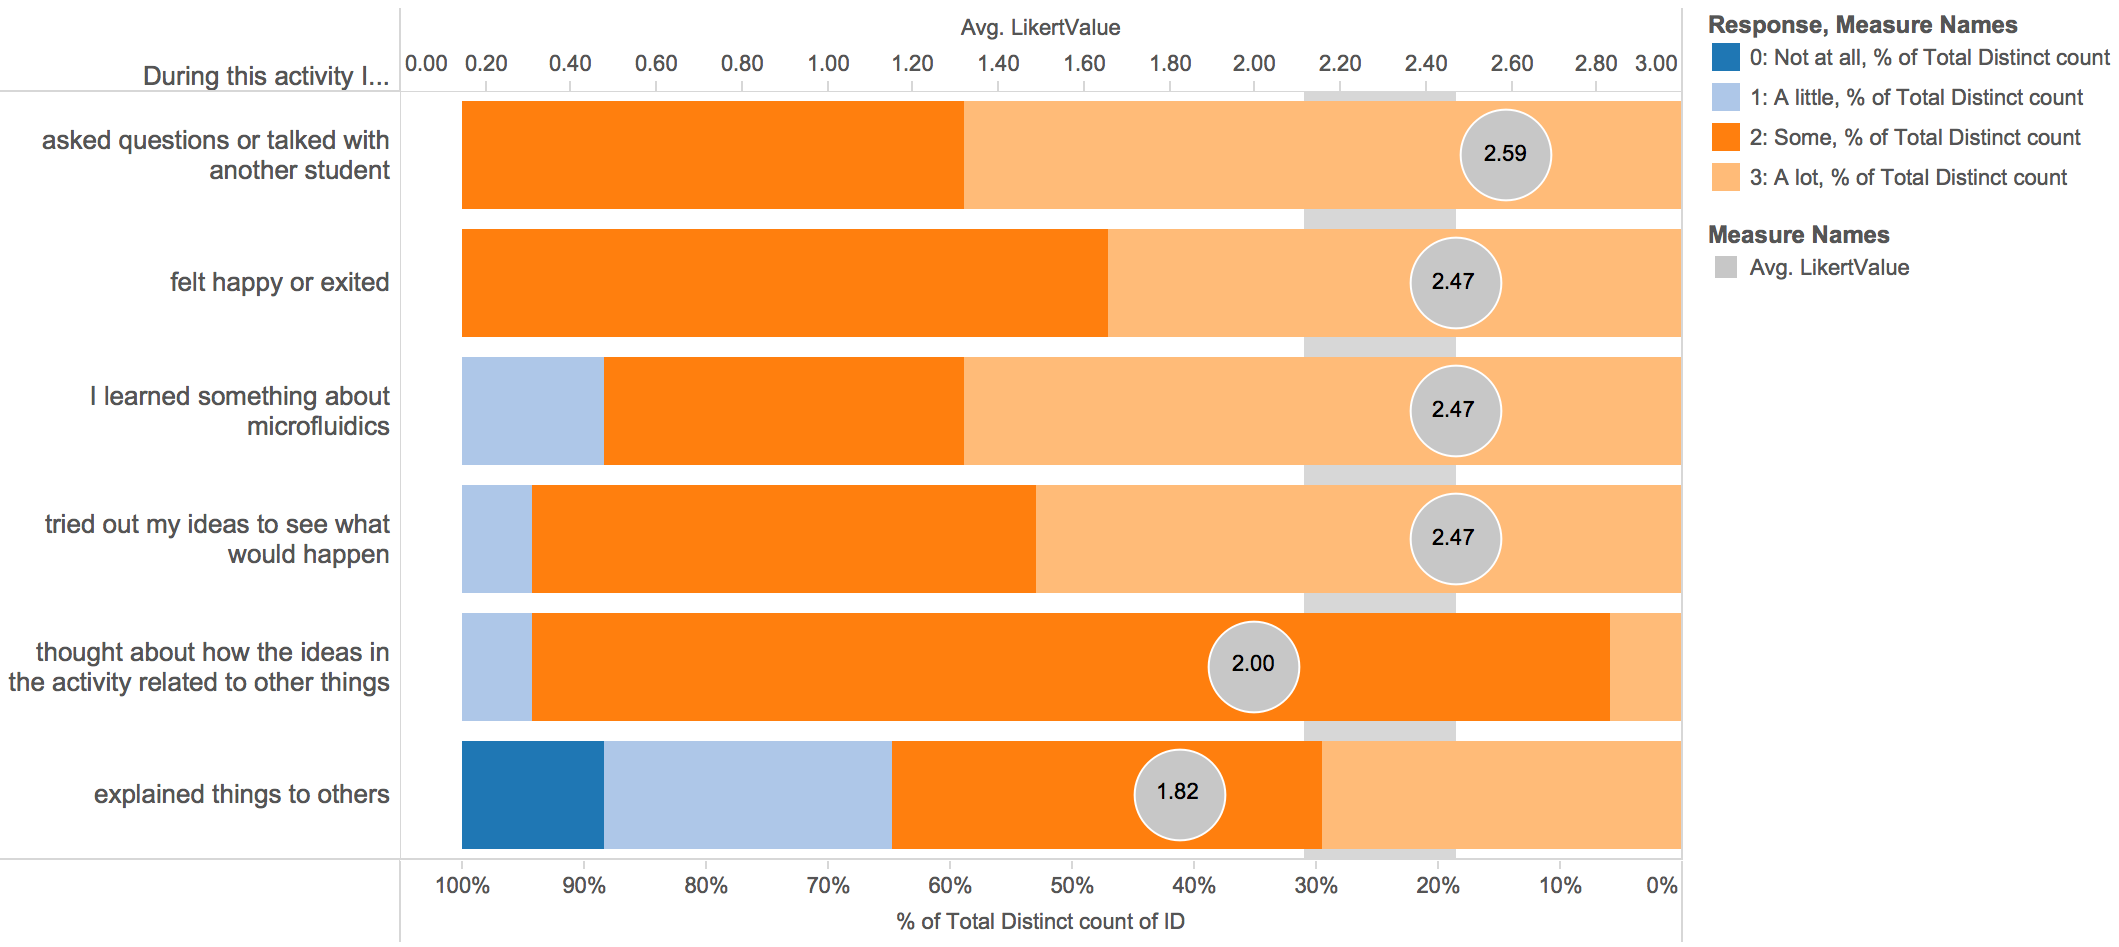
\includegraphics[width=5.9in]{/EduFig1.png}
\caption[\textbf{Responses to section of survey that evaluated student engagement, collaboration, and learning.}]{\textbf{Responses to section of survey that evaluated student engagement, collaboration, and learning.} Survey questions were all phrased with "during this activity I" and followed with responses listed in each row. The legend on the right of the figure describes the response students gave to the question. The average Likert value of each question is displayed in a gray circle. The vertical gray bar running through each row is the standard deviation from the mean for the responses to all questions displayed.}
\label{figure:EduFig1}
\end{figure}
\FloatBarrier

The second section of the survey was designed to evaluate whether the activity was appropriate for the students that were involved in it \ref{figure:EduFig2}. The students were asked whether their participation was voluntary to which all but one responded that they wanted to be involved as opposed to being forced into the activity. The second and third questions probe more directly whether the students had an appropriate level of knowledge and skill coming into the activity to make it beneficial for them. The second question, which asked how much the students knew about the subject indicated that they have all some experience in the subject area, which is to be expected as all students were concurrently enrolled in a college-level microfluidics course. The final question directly asked the students if they thought the activity was at the appropriate skill level for them. Approximately 80\% of students said that it was appropriate for their skill and knowledge level, while the rest responded that it was too easy for them. No students responded that the activity was too difficult for them. These three questions indicate that the activity may have been too easy to accomplish for students in a microfluidics class but the high percentage of students that responded they were doing the activity because they wanted to was high, indicating they still found the activity enjoyable. 

\begin{figure}[h!] %DONE
\centering
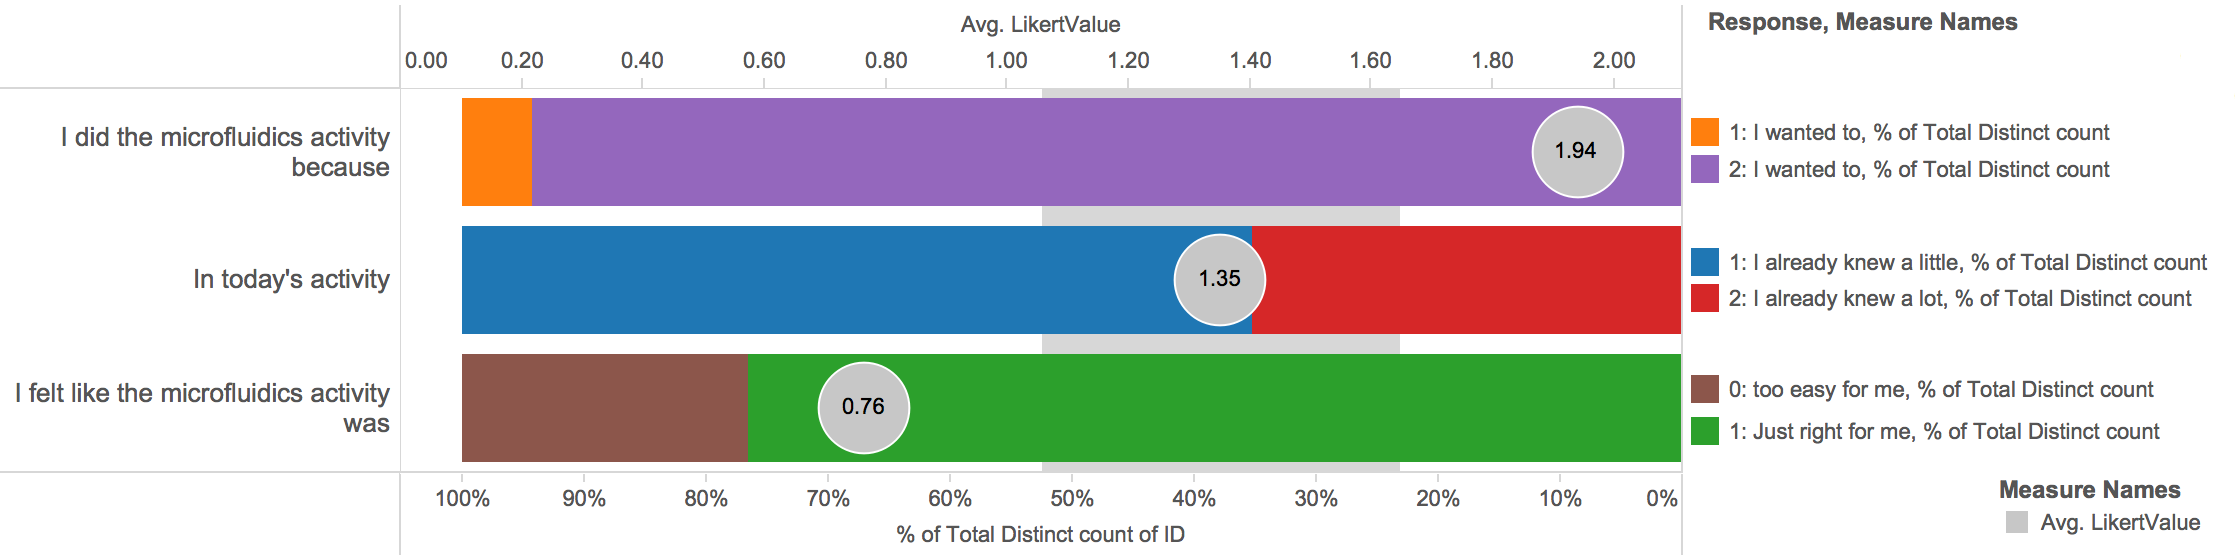
\includegraphics[width=5.9in]{/EduFig2.png}
\caption[\textbf{Response to section of survey to measure appropriateness of microfluidic blocks activity for the students participating in the activity}]{\textbf{Response to section of survey to measure appropriateness of microfluidic blocks activity for the students participating in the activity} Each row represents the responses to a question posed in the survey. The options given to respond to each question are unique and are indicated by color in the chart and to the legend to the right of each bar. The mean Likert value for each question is displayed in grey and placed at the mean of the responses for each question.}
\label{figure:EduFig2}
\end{figure}


The third set of questions asked the students who participated in the activity whether they thought that the open microfluidic blocks were well suited as an educational tool/toy and if they thought it would make a good research prototyping tool (Fig \ref{figure:EduFig3}). The feed back for all questions in this segment were highly positive. The first question, which asked if they thought the platform would make for a good prototyping tool in lab demonstrates that the do see practical applications for the platform beyond what they experienced in the activity they were participating in. The second question asked if the students thought that open microfluidic blocks were useful as a teaching tool, giving additional feedback on what they thought about the activity they had just participated in. The third question asked how they felt about open microfluidic blocks as a learning tool/toy that could be used and experienced at home. The positive response given here suggests that they found the blocks easy enough to use that direct supervision from an instructor while using the platform is unnecessary would be comfortable creating microfluidic circuits at home.

\begin{figure}[h!] %DONE
\centering
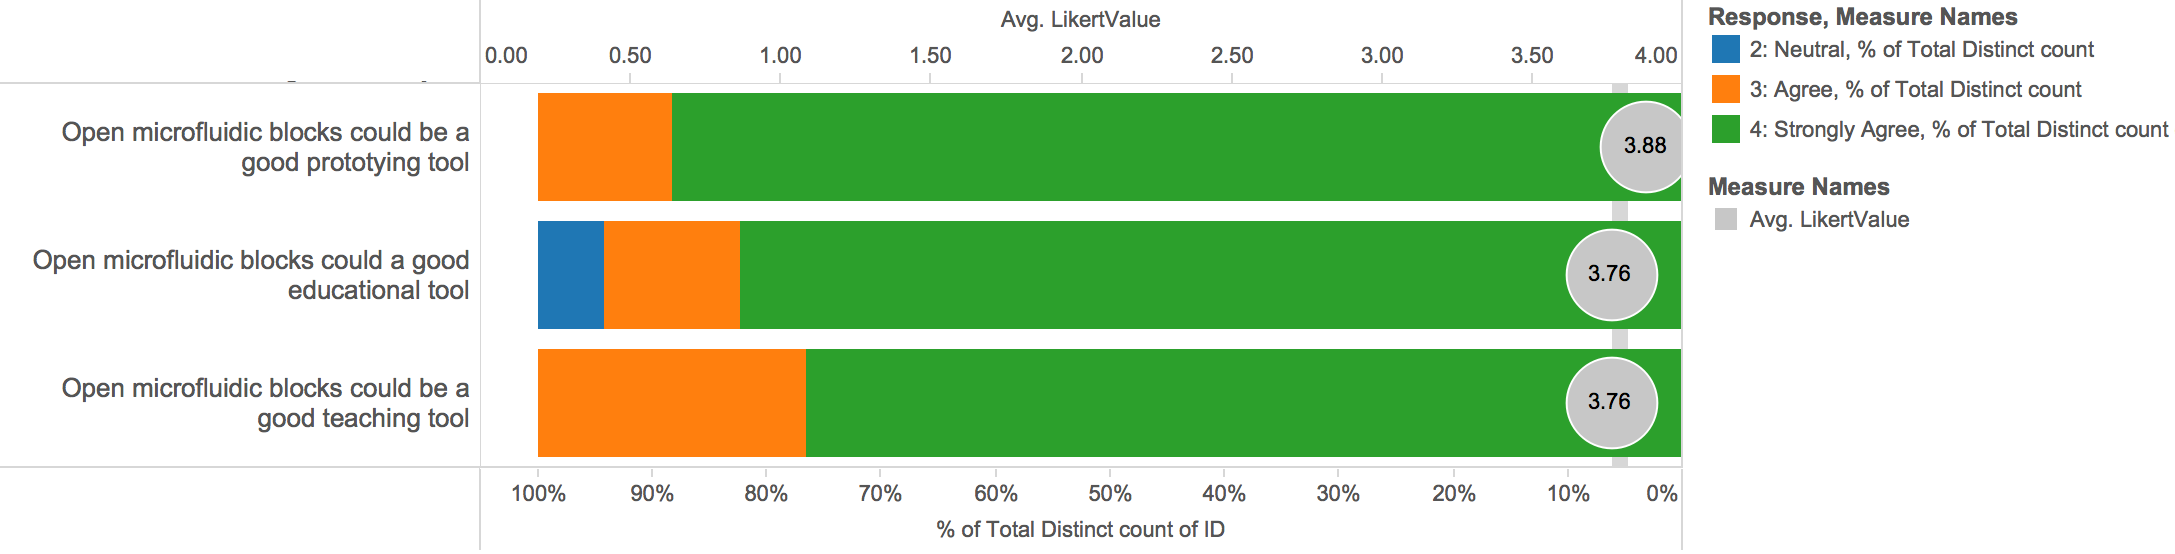
\includegraphics[width=5.9in]{/EduFig3.png}
\caption[\textbf{Response to section of survey how students felt about the practical value of the open microfluidic blocks platform}]{\textbf{Response to section of survey how students felt about the practical value of the open microfluidic blocks platform} The questions asked in this section of the survey were Do you think that... "open Microfluidic blocks could be a good teaching tool in the classroom?", "open microfluidic blocks could be a good prototyping tool for research?", and "open microfludic blocks could be a good educational toy in a home or informal learning space?". Responses were measured from 0 as "strongly disagree" to 4 as "strongly agree". The mean Likert Values for each questions is in grey and overlayed on mean response to each question asked. The mean Likert value for all questions in this section is a vertical grey bar that goes through all rows.}
\label{figure:EduFig3}
\end{figure}

\section{Conclusions and future work}
The responses to the survey were consistently positive and show that the platform has great potential as a learning to to engage and teach microfluidics in the classroom and beyond. The sample sized used in this study was relatively small and focused on a very small subset of individuals, those currently enrolled in a college-level microfluidics class. To address this limited sample size we are currently working with the Discovery Outreach program to test the platform and activity on students elementary to high school. The activity will need to be tailored to fit the group experiencing it, but it will integrate well with the established microfluidics activities that Discovery Outreach is already hosting. We hope that by reaching a larger sample size we will be able to discover flaws in the platform and make improvements to it to not only make it more robust but to improve learning outcomes from students working with the microfluidic blocks. We also did not survey for the effectiveness of the cross sectional open microfluidics device along with the brief explanation of the Generalized Cassie Law. Future studies will include those components to determine how useful they are to students if they are useful at all.

A goal of this study was to create a tool that allowed good student engagement, good learning outcomes, but with minimal preparation to the instructor, and at minimal cost. The open microfluidic blocks used in this study were 3D printed and delivered to us from a service. 3D printing technology makes this platform highly accessible for individuals and institutions around the country and world. The resin used in printing these parts, Accura 25, is fairly hydrophobic, however, there are more hydrophilic resins available for printing which eliminate the need for plasma treatment (a technique with a relatively high cost of investment) of the blocks before use. The blocks were also designed to be compatible with injection molding techniques so that mass production of the platform is feasible which would considerably lower the cost-of-entry for access to the blocks. 

Our ultimate goal with the open microfluidic blocks platform is to create a tool that not only engages people, and helps them learn, but to make microfluidics fun, to make it a subject that individuals want to learn more about. If these results we achieved in this pilot study continue to receive the same feedback as the sample size and scope is expanded we will be well on our way from turning microfluidics from a dirty word into something people are excited about.

\section{Acknowledgements}
We would like to thank Dr. Yan Wu for organizing the microfluidics learning event, without that, this endeavor would have never been possible, Jay Ludden for introducing the idea of educational outreach as an use for the open microfluidic blocks, as well as vetting the survey questions and assembling the lesson plan, and Travis Tangen of Discovery Outreach for his valuable expertise and input in educational outreach.

\begin{figure}[h!] %DONE
\centering
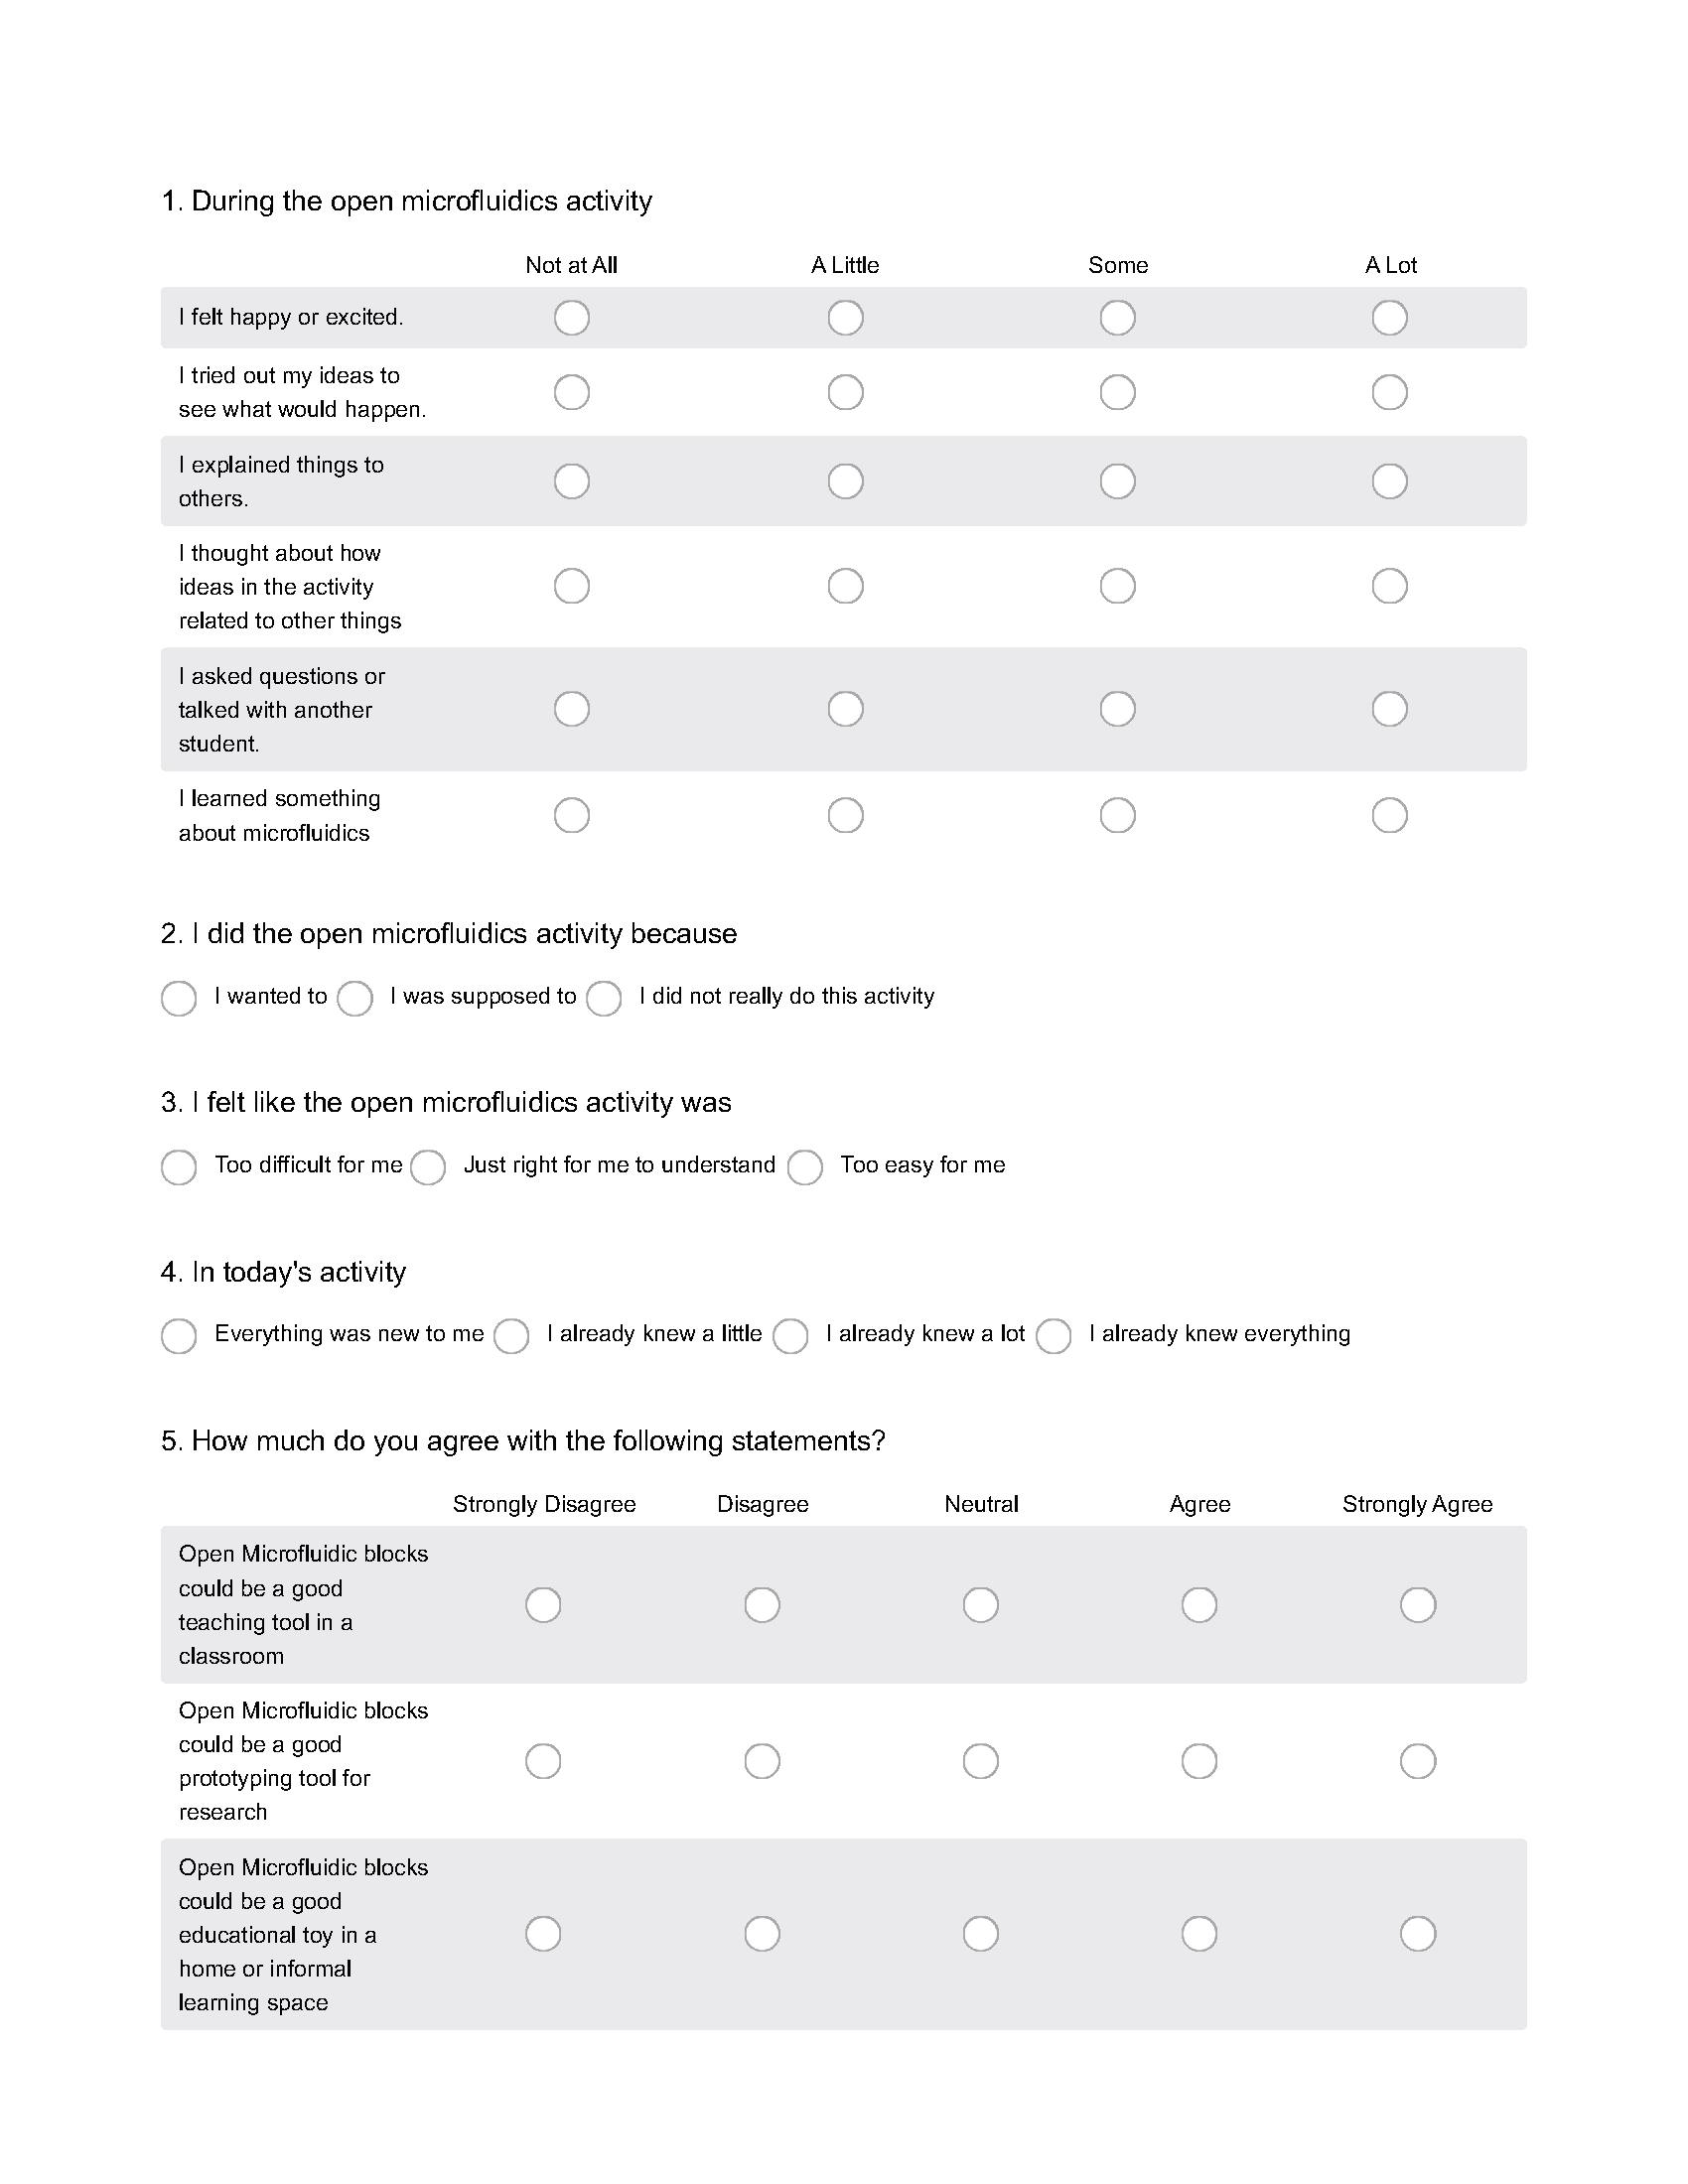
\includegraphics[width=6in]{/survey.png}
\caption[\textbf{Survey for open microfluidic blocks activity}]{\textbf{Survey for open microfluidic blocks activity}}
\label{figure:survey}
\end{figure}







\chapter{Surface-tension driven open microfluidic platform for hanging droplet culture}
\label{App:HangingDroplet}

\begin{figure}[ht] %DONE
\centering
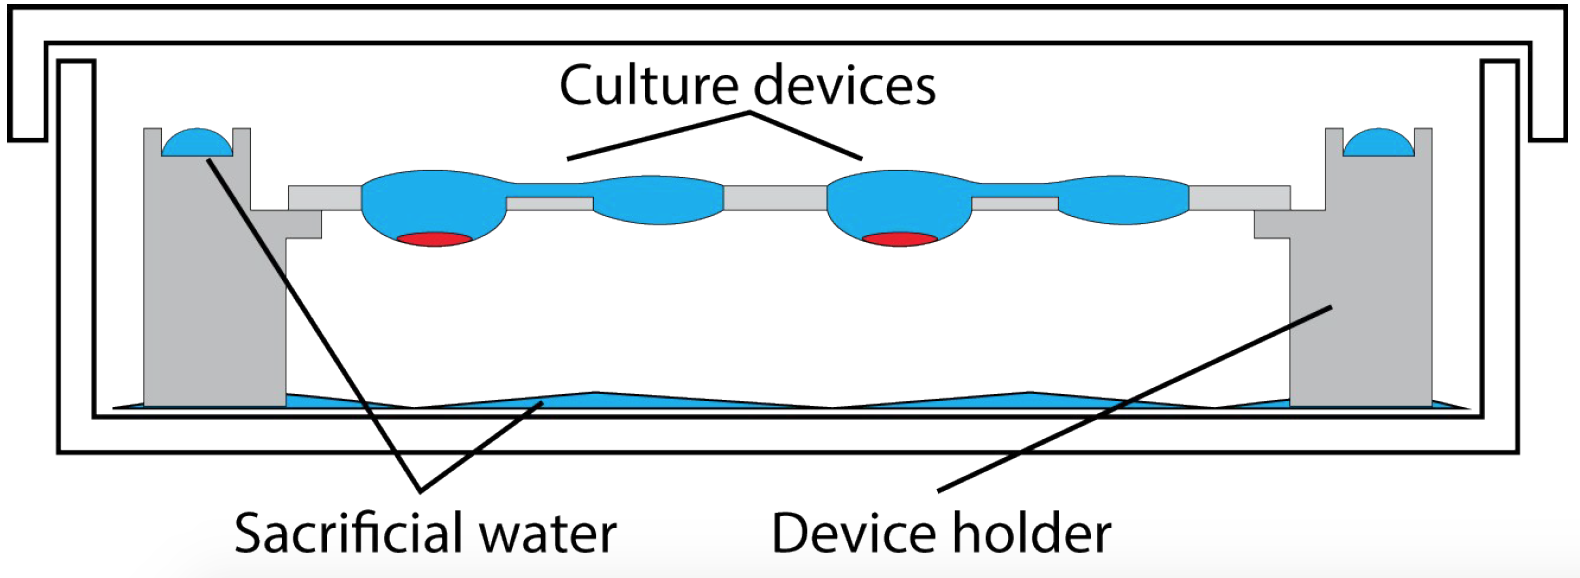
\includegraphics[width=4.5in]{/FigS1.png}
\caption{The device holder is placed in an OmniTray (Nunc) water is added to the bottom of the OmniTray and to the channel features of the device holder. The device is then placed into the device holder and filled with mediaand cells. The lid is placed on the OmniTray to ensure proper humidification of the device to prevent evaporation.}
\label{figure:FigS1}
\end{figure}

\begin{figure}[ht] %DONE
\centering
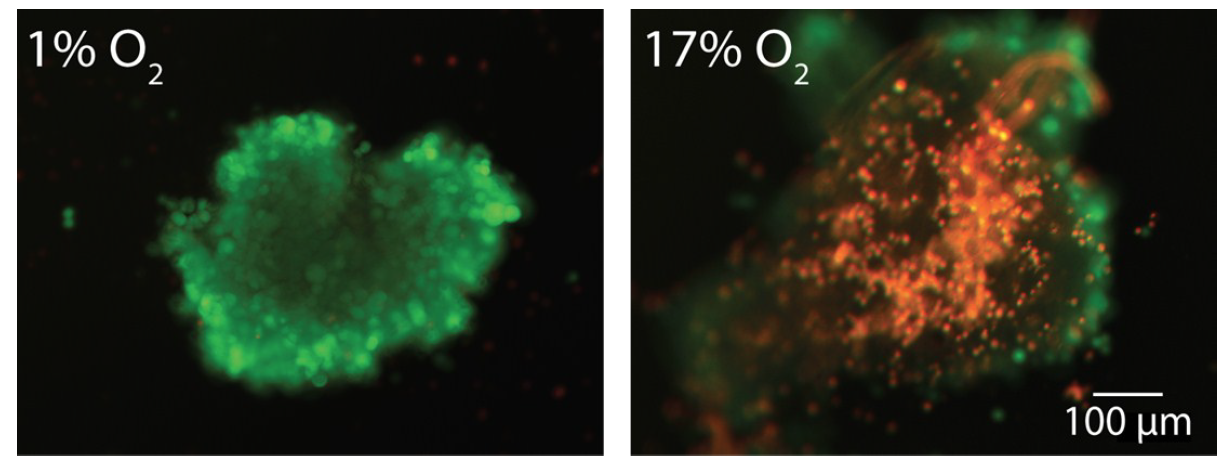
\includegraphics[width=4.5in]{/FigS2.png}
\caption{10,000 MDA-MB-231 cells were seeded into the culture well of the device and were cultured at either normoxic or hypoxic conditions for 48 hours before imaging. Live cells (green) were strained with calcein AM and dead cells were strained with ethidium homodimer (red). Spheroids were extracted from the device and transferred to a well plate for imaging. The hypoxic condition formed a markedly smaller spheroid with no low viability core, while the normoxic condition formed a spheroid with a low-viability, hypoxic core typical of what hasbeen previously observed}
\label{figure:FigS2}
\end{figure}

\begin{figure}[ht] %DONE
\centering
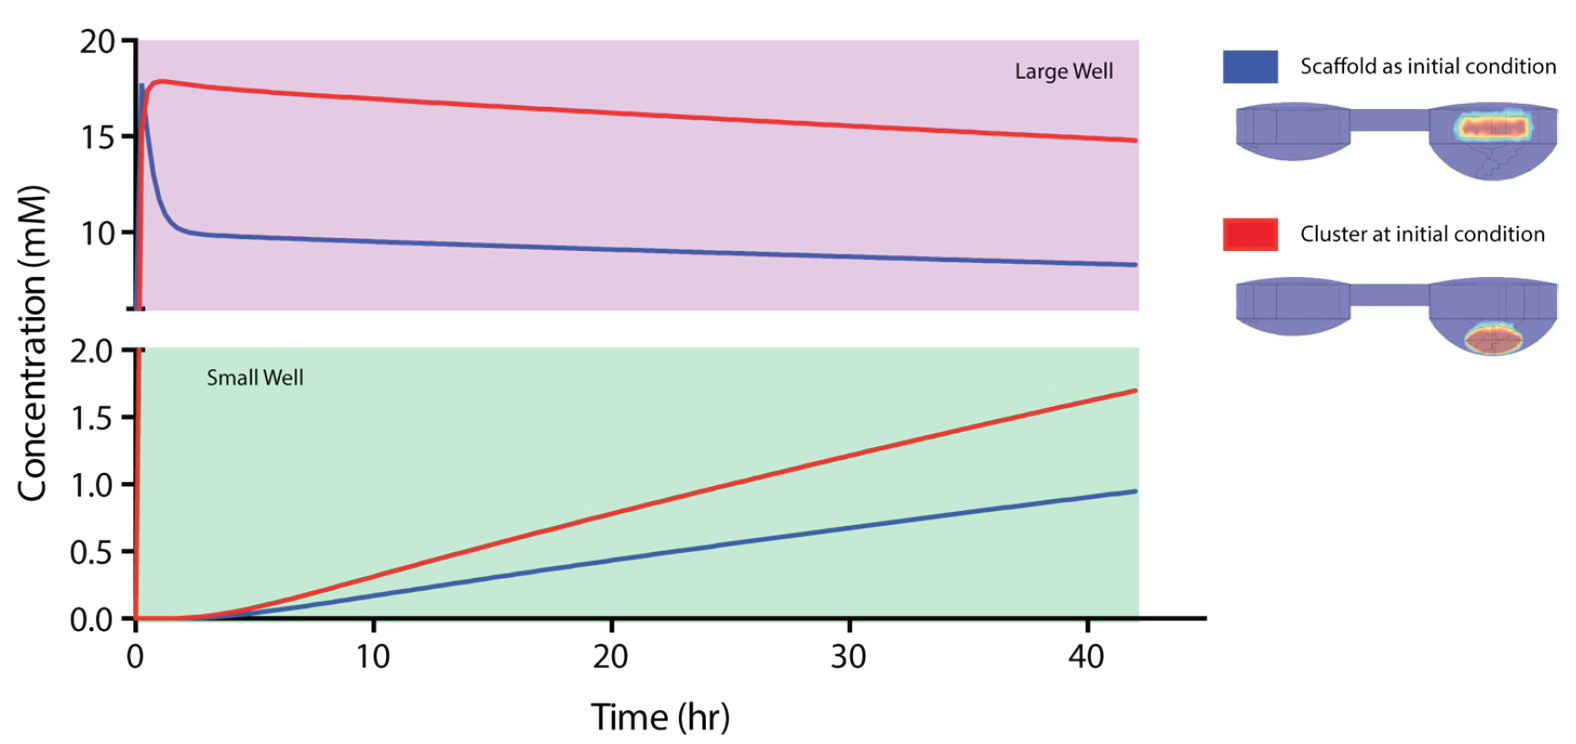
\includegraphics[width=4.5in]{/FigS3.png}
\caption{The average concentration in the bottom meniscus of each well following solute release in a modeled bone-like scaffold or cluster in the culture well.}
\label{figure:FigS3}
\end{figure}

\begin{singlespacing}
\setlength\bibitemsep{2.0\itemsep}
\printbibliography
\end{singlespacing}


\end{document}






















































































